\chapter{Theoretical Background}

\lettrine[
	nindent=0em, findent=0.5em, loversize=-0.12, lines=5
]{\initfamily{D}}{\bfseries\color{Blue}eep learning}\index{Deep learning},
\emph{a class of \acrlong{ml}\index{Machine learning} algorithms based on
\acrlongpl{nn}}, has revolutionized the way we tackle a problem from a \gls{ml}
perspective and is one if not the most important factor for recent \gls{ml}
achievements. Solving complex tasks such image classification\index{Image
classification} or language translation\index{Language translation}, that for
years have bedevilled traditional \gls{ml} algorithms, constitutes the signature
of \gls{dl}. Admittedly, \emph{the advent of a deep
\acrlong{cnn}\index{Convolutional neural network}}, the AlexNet \parencite{alexnet}
on September 30 of 2012, signified the ``modern birthday'' of this field. On
this day, AlexNet\index{AlexNet} not only won the ImageNet \parencite{Deng_2009}
\gls{ilsvrc}, but dominated it, achieving a top-5 accuracy\index{Top-5 accuracy}
of \SI{85}{\percent}, surpassing the runner-up which achieved a top-5 accuracy
of \SI{75}{\percent}.  AlexNet showed that \glspl{nn} are not merely a
pipe-dream, but they can be applied in real-world problems. It is worth to
notice that ideas of \glspl{nn} trace back to 1943, but it was until recently
that these ideas got materialized. The reason for this recent breakthrough of
\gls{dl} (and \gls{ml}) is twofold. First, the availability of large
datasets\index{Dataset}---the era of big data\index{Big data}---such as
ImageNet\index{ImageNet}. Second, the increase in computational power, mainly of
\acrshortpl{gpu} for \gls{dl}, accelerating the training of deep \glspl{nn} and
traditional \gls{ml} algorithms.

\section{Machine Learning Preliminaries}

Since \gls{dl} is a subfield of \gls{ml}, it is necessary to familiarize with
the later before diving into the former. In this section, the necessary
theoretical background and jargon of \gls{ml} is presented. \Acrlong{ml} can be
defined as \emph{``the science and (art) of programming computers so they can
learn from the data''} \parencite{ml}. A more technical definition is the following:

\begin{definition}[name={Machine learning, \cite{mitchell}}]
	A computer program is said to learn from experience\index{Experience}
	\textbf{E} with respect to some class of tasks\index{Task} \textbf{T} and some
	performance measure \textbf{P}\index{Performance measure}, if its
	performance on \textbf{T}, as measured by \textbf{P}, improves with
	experience \textbf{E}.
\end{definition}

For instance, a computer program\index{Spam filter} that classifies emails into
spam and non-spam (the task \textbf{T}), can improve its accuracy, i.e. the
percentage of correctly classified emails (the performance \textbf{P}), through
examples of spam and non-spam emails (the experience \textbf{E}). But in order
to take advantage of the experience aka \emph{data}\index{Data}, it must be
written in such a way that \emph{adapts to the patterns in the data}. Certainly,
a \emph{traditional spam filter can not learn from experience}, since the latter
does not affect the classification rules of the former and as such, its
performance. For a traditional spam filter to adapt to new patterns and perform
better, it must change its hard-wired rules, but by then it will be a different
program. In contrast, a \emph{\gls{ml}-based filter can adapt to new patterns,
simply because it has been programmed to do so}. In other words, \emph{in
traditional programming\index{Traditional programming} we write rules for
solving \textbf{T} whereas \textbf{in \gls{ml} we write rules to learn the
rules} for solving \textbf{T}}. This subtle but essential difference is what
gives \gls{ml} algorithms the ability to take advantage of the data.

\subsection{Learning paradigms}
\label{subsec:paradigms}

Depending on the type of experience they are allowed to have during their
\emph{training phase}\index{Training phase} \parencite{deeplearning}, \gls{ml}
approaches are divided into three main \emph{learning paradigms}\index{Learning
paradigms}: \emph{\textbf{unsupervised learning}\index{Unsupervised learning},
\textbf{supervised learning}\index{Supervised learning} and
\textbf{reinforcement learning}\index{Reinforcement learning}}. The following
definitions are not by any means formal, but merely serve as an intuitive
description of the different paradigms.

\begin{definition}[name=Unsupervised learning]
	The experience comes in the form $\dtrain = \{\vcx_i\}$, where $\vcx_i \sim
	p(\vcx)$ is the input\index{Input} of the $i$-th training
	instance\index{Training instance} aka sample\index{Training sample}. In this
	paradigm we are interested in learning useful properties of the underlying
	structure captured by $p(\vcx)$ or $p(\vcx)$ itself.
\end{definition}

For example, suppose we are interested in generating images that look like
Picasso paintings. In this case, the input is just the pixel values, i.e.  $\vcx
\in \mathbb{R}^{W \times H \times 3}$. The latter follow a distribution
$p(\vcx)$, so all we have to do is to train an unsupervised learning algorithm
with many Picasso paintings to get a \emph{model}, that is $\hat{p}(\vcx)$.
Assuming the estimation of the original distribution is good enough, new
realistically looking paintings (with respect to original Picasso paintings) can
be ``drawn'' by just sampling from $\hat{p}(\vcx)$. In the ML parlance, this
task is known as \emph{generative modeling}\index{Generative modeling} while
inputs are also called \emph{features, predictors or
descriptors}\index{Feature}\index{Descriptor}\index{Predictor}.

\begin{definition}[name=Supervised learning]
	The experience comes in the form $\dtrain = \{(\vcx_i, \vcy_i)\}$, where
	$(\vcx_i, \vcy_i) \sim p(\vcx, \vcy)$ and $\vcy_i$ is the
	output\index{Output} aka label\index{Label} of the $i$-th training instance.
	In this paradigm we are usually interested in learning a function $f \colon
	\mcl{X} \to \mcl{Y}$.
\end{definition}

This paradigm comes mainly under two flavors: \emph{regression\index{Regression}
and classification\index{Classification}}, which are schematically depicted in
\Figure{} \ref{fig:supervised_learning}. In regression the interest is in
predicting a continuous value given an input, i.e.  $y \in \mathbb{R}$, such as
a molecular property given a mathematical representation of a molecule. In
classification, the interest is to predict in which of $k$ classes an input
belongs to, i.e. $y \in \{1, \ldots, k\}$, such as predicting the breed of a dog
image given the raw pixel values of the image. The term ``supervised'' is coined
due to the ``human supervision'' the algorithm receives during its training
phase\index{Training phase}, through the presence of the correct answer (the
label) in the experience.  In a sense, in this paradigm we ``teach'' the
learning algorithm aka \emph{learner}. It should be emphasized that the label is
not constrained to be single-valued, but can also be multi-valued. In this case,
one talks about \emph{multi-label regression\index{Multi-label regression} or
classification\index{Multi-label classification}} \parencite{Read_2009}.

A more exotic form of supervised learning is \emph{conditional generative
modelling}\index{Conditional generative modelling}, where the interest is in
estimating $p(\vcx \mid \vcy)$. For example, one may want to build a model that
generates images of a specific category or a \emph{model that designs
molecules/materials with tailored properties} \parencite{Kim2018, Yao2021,
Gebauer2022}. This is one approach of how \gls{ml} can tackle the \emph{inverse
design problem}\index{Inverse design} in chemistry\index{Chemistry}.

\begin{figure}
	\centering
	\begin{subfigure}[b]{0.49\textwidth}
		\centering
		\begin{tikzpicture}
			\pgfmathsetseed{1}
			\begin{axis}[
					thick, ticks=none, mark size=1.2pt,
					xmin=0, xmax=1.1, ymin=0, ymax=1,
					xlabel=$x_1$, ylabel=$x_2$,
				]
				\coordinate (start) at (0.62, 0);
				\coordinate (stop) at (0.2, 1);
				\coordinate (xmax-ymin) at (1.1, 0);
				\coordinate (xmin-ymin) at (0, 0);
				\coordinate (xmin-ymax) at (0, 1);
				\coordinate (xmax-ymax) at (1.1, 1);
				\addplot+ [
					only marks, samples=20, variable=\t, domain=0:1,
				] ({exp(-0.55*t^2) + 0.01*rnd}, {0.6*rnd});
				\addplot+ [
					only marks, samples=20, variable=\t, domain=0.4:1, mark=*,
				] ({exp(-5*t^2) + 0.05*rnd}, {0.8*rnd});
				% y = -2.381x + 1.476
				\addplot [samples=2, black, dashed, ultra thick] {-2.381*x + 1.476};
				% y = -3.381x + 1.476
				\addplot [samples=2, black, ultra thick] {-5.581*x + 2.976};
				\legend{,,Model, True $f$};
			\end{axis}
		\end{tikzpicture}
		\caption{Classification.}
		\label{fig:classification}
	\end{subfigure}
	\begin{subfigure}[b]{0.49\textwidth}
		\begin{tikzpicture}
			\centering
			\pgfmathsetseed{1}
			\begin{axis}[
					thick, xlabel=$x_{\phantom{1}}$, ylabel=$y$, domain=-2:2,
					legend pos=north west, ticks=none,
				]
				\addplot [
					only marks, samples=12,
					mark options={fill=blue!20, mark size=2.5pt,}
				] {x^2 + x^3 + 2*rnd};
				\addplot [no marks, dashed, ultra thick, samples=20] {x^2 + 0.1*x^3 + 0.1*x};
				% The true function
				\addplot [no marks, ultra thick, samples=20] {x^2 + x^3 + 0.5};
				\legend{,Model, True $f$};
			\end{axis}
		\end{tikzpicture}
		\caption{Regression.}
	\end{subfigure}
	\caption{Main tasks of supervised learning.}
	\label{fig:supervised_learning}
\end{figure}

\begin{definition}[Reinforcement learning]
	The experience comes from the interaction of the learner, called
	agent\index{Agent} in this context, with its environment. In other words,
	there is a feedback loop between the learner and its environment. In this
	paradigm we are interested in building an agent that can take suitable
	actions in a given situation.
\end{definition}

The agent observes its \emph{environment}, selects and performs \emph{actions}
and gets \emph{rewards or penalties} in return. The goal is to learn an optimal
strategy, called a \emph{policy}, that \emph{maximizes the long-term reward}
\parencite{ml}. A policy simply defines the action that the agent should
choose in a given situation. In contrast to supervised learning, where the
correct answers are provided to the learner, \emph{in reinforcement learning the
learner must find the optimal answers by trial and error}
\parencite{bishop2007}. Reinforcement learning techniques find application in
fields such as gaming (AlphaGo is a well known example), robotics, autonomous
driving and recently chemistry \parencite{li, Gow2022}. Since in the present
thesis only supervised learning techniques were employed, the remaining of this
chapter is devoted to this learning paradigm.

\subsection{Formulating the problem of supervised learning}
\label{subsec:supervised_learning}

The general setting of supervised learning is as follows: we assume that there
is some relationship between $\vcx$ and $\vcy$:
\begin{equation}
	\label{eq:supervised}
	\vcy = f(\vcx) + \vc{\epsilon}
\end{equation}
and we want to estimate $f$ from the data. The function $f$ represents the
\emph{systematic information} that $\vcx$ gives about $\vcy$ while
$\vc{\epsilon}$ is a \emph{random error term}\index{Random error term}
independent of $\vcx$ and with zero mean. More formally, we have an input space
$\mcl{X}$, an output space $\mcl{Y}$ and we are interested in learning a
function $\hat{h} \colon \mcl{X} \to \mcl{Y}$, called the
\emph{hypothesis}\index{Hypothesis}, which produces an output $\vcy \in \mcl{Y}$
given an input $\vcx \in \mcl{X}$.  At our disposal we have a collection of
input-output pairs $(\vcx_i, \vcy_i)$, forming the \emph{\textbf{training
set}}\index{Training set} denoted as $\dtrain$, with the pairs drawn
\acrshort{iid} from $p(\vcx, \vcy)$.

Ideally, we would like to learn a hypothesis that minimizes the
\emph{\textbf{generalization error or loss}}\index{Generalization
error}\index{Generalization loss}:
\begin{equation}
	\label{eq:generalization_loss}
	\loss \coloneqq
	\int_{\mcl{X} \times \mcl{Y}} \ell(h(\vcx), \vcy) p(\vcx, \vcy) d\vcx d\vcy
\end{equation}
that is, the expected value of some \emph{loss function}\index{Loss function}
$\ell$ over all possible input-output pairs. A loss function just measures the
discrepancy of the prediction $h(\vcx) = \hat{\vcy}$ from the true value $\vcy$
and as such, the best hypothesis is the one that minimizes this integral.
Obviously, it is impossible to evaluate the integral in \Equation{}
\ref{eq:generalization_loss}, since in general we don't know the joint
probability distribution $p(\vcx, \vcy)$.

The idea is to use the \emph{training error or loss}\index{Training
error}\index{Training loss}:
\begin{equation}
	\label{eq:training_loss}
	\loss_\text{train} \coloneqq \frac{1}{\lvert \dtrain \rvert} \sum_{i \in \dtrain}
	\ell(h(\vcx_i), \vcy_i)
\end{equation}
as an approximation for the generalization loss, and \emph{choose the hypothesis
that minimizes the training loss}, a principle known as \emph{empirical risk
minimization}\index{Empirical risk minimization}. In other words, to get a
hypothesis aka \emph{model} $\mcl{M}$\index{Model} from the data, we need to
solve the following optimization problem:
\begin{equation}
	\label{eq:problem}
	\hat{h} \gets \argmin_{h \in \mcl{H}} \ltrain
\end{equation}
which is achieved by just feeding the training data into the learning
algorithm $\mcl{A}$\index{Learning algorithm}:
\begin{equation}
	\label{eq:learner}
	\mcl{M} \gets \mcl{A}(\dtrain)
\end{equation}

\subsection{Components of a learning algorithm}

By breaking down \Equation{} \ref{eq:problem}, i.e. the optimization problem the
learner needs to solve, the components of a learner can be revealed. The latter
is comprised of the following three ``orthogonal'' components: \emph{a
\textbf{hypothesis space}\index{Hypothesis space}, a \textbf{loss
function} and an \textbf{optimizer}}. We now look into each of them
individually and describe the contribution of each one to the solution of the
optimization problem. For the ease of notation and clarity, in the remaining of
this chapter we will stick to examples from simple (single-valued) regression
and binary classification.

\begin{definition}[Hypothesis space]
	The set of hypotheses (functions), denoted as $\mcl{H}$, from which the
	learner is allowed to pick the solution of \Equation{} \ref{eq:problem}.
\end{definition}

A simple example of a hypothesis space, is the one used in univariate
\emph{linear regression}\index{Linear regression}:
\begin{equation}
	\label{eq:linear}
	\hat{y} = b + w x
\end{equation}
where $\mcl{H}$ contains all lines (or hyperplanes in the multivariate case)
defined by \Equation{} \ref{eq:linear}. Of course, one can get \emph{a
more expressive} hypothesis space, by including polynomial terms, e.g.:
\begin{equation}
	\label{eq:polynomial}
	\hat{y} = b + w_1 x + w_2 x^2
\end{equation}
The more expressive the hypothesis space, the larger the
\emph{\textbf{representational capacity}}\index{Representational capacity} of
the learning algorithm. For a formal definition of representational capacity,
the interested reader can look at \emph{Vapnik-Chervonenkis
Dimension}\index{Vapnik-Chervonenkis dimension} \parencite{Hastie2009}.

\begin{definition}[Loss function]
	A function that maps a prediction into a real number, which intuitively
	represents the quality of a candidate hypothesis.
\end{definition}

For example, a typical loss function used in regression is the \emph{squared
loss}\index{Squared loss}:
\begin{equation}
	\label{eq:squared_loss}
	\ell(\hat{y}, y) \coloneqq (\hat{y} - y)^2
\end{equation}
where $y, \hat{y} \in \mathbb{R}$. A typical loss function for binary
classification is the \emph{binary cross entropy
loss}\index{Binary cross entropy loss}:
\begin{equation}
	\label{eq:cross_entropy}
    \ell(\hat{y}, y) \coloneqq
    - \left[ y \cdot \log (\hat{y})
    + (1 - y) \cdot \log (1 - \hat{y}) \right]
\end{equation}
where $y \in \{0, 1\}$, indicating the correct class, and $\hat{y} \in [0, 1]$
which corresponds to the predicted probability for class-$1$. Notice that in
both cases the loss is minimum when the prediction is equal to the ground truth.
For the cross entropy loss, if $y=1$ is the correct class, then the model must
predict $\hat{y}=1$ for the loss to be minimized.

\label{subsec:regularization}
Usually, we are not only penalizing a hypothesis for its mispredictions, but
also for its \emph{complexity}. This is done in purpose, since a learner with a
\emph{very rich hypothesis space} can easily memorize the training set but fail
to generalize well to new unseen examples. \emph{Every modification that is made
to a learner in order to reduce its generalization loss but not its training
loss, is called \textbf{regularization}}\index{Regularization} \parencite{deeplearning}.

A common---but not the only---way to achieve that, is by including another
penalty term called \emph{regularization term or
\textbf{regularizer}}\index{Regularizer}, denoted as $\mcl{R}$, in \Equation{}
\ref{eq:training_loss}:
\begin{equation}
	\label{eq:regularization}
	\loss_\text{train} \coloneqq \frac{1}{\lvert \dtrain \rvert} \sum_{i \in \dtrain}
	\ell(\hat{\vcy}_i, \vcy_i)
	+
	\lambda \mcl{R}
\end{equation}
The $\lambda$ factor controls the strength of regularization and it is an
\emph{\textbf{hyperparameter}}\index{Hyperparameter}, i.e. a parameter that is
not learned during training but \emph{whose value is used to control the
training phase\index{Training phase}.} In order to see how $\lambda$ penalizes
model complexity, assume we perform univariate polynomial
regression\index{Polynomial regression} of degree $k$:
\begin{equation}
	\hat{y} = b + \sum_{i=1}^k w_i x^i
\end{equation}
combining \gls{msl}\index{Mean squared loss} and \emph{lasso
regularization}\index{Lasso regularization} as training loss:
\begin{equation}
	\label{eq:lasso}
	\loss_\text{train} = \frac{1}{\lvert \dtrain \rvert} \sum_{i \in \dtrain}
	\ell(\hat{y}_i - y_i)^2
	+
	\lambda \sum_{i=1}^k \lvert w_i \rvert
\end{equation}
Let's apply a very strong regularization by setting $\lambda \to \infty$ (in
practice we set $\lambda$ to a very large value) and observe what happens to the
\emph{weights}\index{Weights} $w_i$. By setting $\lambda \to
\infty$, the regularization term dominates the \gls{msl} and as such, the only
way to minimize the training loss is by setting $w_i = 0$. This leave us
with a very simple model---only the \emph{bias}\index{Bias} term $b$
survives---which always predicts the mean value of $y$ in the training set.

Applying a regularizer\index{Regularizer}, is also useful when we need to select
between two (or more) competing hypotheses that are equally good. For example,
assuming two hypotheses achieve the same (unregularized) training loss, the
inclusion of a regularization term help us decide between the two, \emph{by
favoring the simplest one}. This is reminiscent of the \emph{\textbf{Occam's
razor} aka \textbf{principle of parsimony}}\index{Occam's razor}\index{Principle
of parsimony}, which advocates that between two competing theories with equal
explanatory power, one should prefer the one with the fewest assumptions.

\begin{definition}[Optimizer]
	An algorithm that searches through $\mcl{H}$ for the solution of \Equation{}
	\ref{eq:problem}.
\end{definition}

Having defined the set of candidate models (the hypothesis space) and a measure
that quantifies the quality of a given model (the loss function), all that is
remaining is a tool to scan the hypothesis space and pick the model that
minimizes the training loss (the optimizer). A naive approach is to check all
hypotheses in $\mcl{H}$ and then pick the one that achieves the lowest training
loss. This approach can work if $\mcl{H}$ is finite, but obviously doesn't scale
in the general case where $\mcl{H}$ is infinite\footnote{It is not
uncommon for $\mcl{H}$ to be infinite. Even for simple learners like linear
regression $\mcl{H}$ is infinite, since there infinite lines defined by \Equation{}
\ref{eq:linear}.}. More efficient approaches are needed if we are aiming to solve
\Equation{} \ref{eq:problem} in finite time.

One optimizer that is frequently used in \gls{ml} and is the precursor of more
refined ones, is \emph{\textbf{gradient descent}}\index{Gradient descent}. With
this method, the exploration of hypothesis space\footnote{We have implicitly
assumed that $\mcl{H}$ can be parameterized, i.e. $\mcl{H} = \{h(\vcx;\vcth)
\mid \vcth \in \Theta\}$, where $\Theta$ denotes the parameter space, the set of
all values the parameter $\vcth$ can take. This allows us to write the training
loss as function of model parameters and optimize them with gradient descent.}
involves the following steps:

\begin{algorithm}[H]
	$\vcth \gets$ random initialization\;
	\While{stopping criterion not met}{
		$\vcth \gets \vcth - \eta \nabla_{\vcth}\ltrain(\vcth)$\; 
	}
	\caption{Gradient descent}
	\label{algo:gd}
\end{algorithm}

\noindent where $\eta$ is a small number called the \emph{learning
rate}\index{Learning rate}. Gradient descent is based on the idea that
if a multivariate function is defined and differentiable at a point $\vcx$, then
$f(\vcx)$ \emph{decreases fastest if one takes a small step from $\vcx$ in the
direction of negative gradient at $\vcx$, $-\nabla f(\vcx)$}.

The motivation becomes clear if we look at the differential of $f(\vcx)$ in
direction $\vc{u}$: \begin{equation} \label{eq:differential} f(\vcx + \delta
\vc{u}) - f(\vcx) = \nabla f(\vcx) \cdot \delta \vc{u} \end{equation} \Equation{}
\ref{eq:differential} says that this differential is minimized\footnote{The
right hand side of \Equation{} \ref{eq:differential} is a dot product.} when
$\delta \vc{u}$ is anti-parallel to $\nabla f(\vcx)$ and that is why we subtract
the gradient in \Algorithm{} \ref{algo:gd}, i.e. move in direction anti-parallel to
the gradient. The fact that \Equation{} \ref{eq:differential} holds only locally
(magnitude of $\delta \vc{u}$ must be small) explains why $\eta$ must be a small
number. It should be added that gradient descent can be trapped to (potential)
local minima of the training loss and therefore fail to solve \Equation{}
\ref{eq:problem}. As it will be discussed later, this is not a problem, because
\emph{the ultimate purpose is to find a hypothesis that generalizes well, not
necessarily the one that minimizes the training loss}\footnote{Remember we use
the training loss (see \Equation{} \ref{eq:training_loss}) as a proxy for the
generalization loss (see \Equation{} \ref{eq:generalization_loss}).}. Optimizers
are discussed in further detail in \Section{} \ref{subsec:nn_training}.

Before moving on, it is worth to add that both the regularization and the
optimizer have an effect on the ``true'' or \emph{\textbf{effective
capacity}}\index{Effective capacity} \parencite{deeplearning} of the learner,
\emph{which might be less than the representational
capacity\index{Representational capacity} of the hypothesis space}. For example
a regularizer penalizes the complexity of an hypothesis, effectively
``shrinking'' the representational capacity of the hypothesis space. The effect
of the optimizer can be understood by looking on its contribution to the
solution of \Equation{} \ref{eq:problem}. As described previously, the optimizer
searches through the hypothesis space. If this ``journey'' is not long enough,
then this ``journey'' is practically equivalent to a long ``journey'' in a
shortened version of the original hypothesis space. In the rest of this chapter,
by the term \emph{\textbf{complexity}\index{Complexity} or
capacity\index{Capacity} of a learner, we mean its effective capacity, which is
affected by all its three components}.

\subsection{Performance, complexity and experience}
\label{subsec:per_com_exp}

Suppose that we have trained our learner, and finally we get our model, as
stated by \Equation{} \ref{eq:learner}. \emph{How can we assess its
performance\index{Performance}?} Remember, we can't calculate the generalization
loss\index{Generalization loss}, since we are not given an infinite amount of
data. First of all, \emph{we should not report the training loss\index{Training
loss}, because it is optimistically biased\index{Optimistically biased}}, as it
is evaluated on the same data that has been trained on\footnote{Intuitively,
this is like assessing students' performance based on problems they have already
seen before. They can easily achieve zero error, just by recalling their
memory.}. What we should is to collect new input-output pairs, forming the
\emph{\textbf{test set}}\index{Test set} $\dtest$, and then \emph{estimate the
generalization loss} as following:
\begin{equation}
	\label{eq:test_loss}
	\loss_\text{test} \coloneqq \frac{1}{\lvert \dtest \rvert} \sum_{i \in \dtest}
	\ell(h(\vcx_i), \vcy_i)
\end{equation}
The \emph{test error or loss}\index{Test error}\index{Test loss} is evaluated on
new---unseen to the learner during the training phase\index{Training
phase}---samples and as such, it is an \emph{unbiased estimate}\index{Unbiased
estimate} of the generalization loss. Usually, since many times is not even
possible to collect new samples, \emph{we split the initial
dataset\index{Dataset} into training and test sets}.

The general recipe for building and evaluating the performance of a \gls{ml}
model has already been presented. What is missing is how we can improve its
performance, or to put it differently, the factors that affect the quality of
the returned model. There are two main factors that determine the performance of
the model: \emph{complexity\index{Complexity} and experience\index{Experience}}.
In general, the larger the experience---the training set---\index{Training set}
the better the performance, just like we humans perform improve on a task by
keep practicing. With regards to the complexity, \emph{learners of low
complexity\index{Low complexity} might fail to capture the patterns in the
data}, meaning that the resulting model will fail to generalize. In contrast,
\emph{learners of higher complexity would be able to capture these patterns},
and as such return models of higher quality. However, \emph{as the complexity of
the learner keeps increasing, the latter is more sensitive to noise, i.e. there
is a higher chance that the learner will simply memorize its experience} and as
such, fail to generalize.

In other words, there is a trade-off between the complexity of the learner and
its performance. The learner should be not too simple but also not too complex,
in order to generalize well. This in turn implies that we need to find a way to
``tune'' the complexity. A common way to achieve that is by using another set of
instances, known as the \emph{\textbf{validation set}\index{Validation set}}. We
train learners of different complexity on the training set\index{Training set},
evaluate their performance on the validation set, and then choose the learner
that performs best on the validation set. The reason we use the validation set
instead of the test set for tuning complexity, is to ensure that the performance
estimation is unbiased. \emph{The test set\index{Test set} should not influence
our decisions in any way}. After we have tuned the complexity, we can estimate
the performance of the resulting model in the test set. Finally, it is a good
practice to retrain the learner on the whole dataset---including validation and
test sets---since more data result in models of higher quality.

\begin{theorem}[%
		Bias-variance decomposition\index{Bias-variance decomposition},
		\cite{Bishop2006}%
	]
	\label{thrm:bias_variance}
    From \Equation{} \ref{eq:supervised} the expected squared loss\index{Squared
    loss}\index{Expected square loss} at $\vcx^*$ can be decomposed as
    following:
	\begin{equation}
		\label{eq:bias_variance}
		\exp{\left(y^* - \hat{f}(\vcx^*)\right)^2}
		=
		\color{blue}\left(f(\vcx^*) - \exp{\hat{f}(\vcx^*)}\right)^2
		\color{black}
		+
		\color{red}\exp{\left(\hat{f}(\vcx^*) - \exp{\hat{f}(\vcx^*)}\right)^2}
		\color{black}
		+
		\sigma_{\epsilon}^{2}
	\end{equation}
	The expected squared loss refers to the average squared loss we would obtain
	by repeatedly estimating $f$ using different training sets, each tested at
	$\vcx^*$. The overall expected squared loss can be computed by averaging the
	left hand side of \Equation{} \ref{eq:bias_variance} over all possible values
	$\vcx^*$.
\end{theorem}

The trade-off between the complexity\index{Complexity} of the learner and its
performance\index{Performance}, is mathematically described in \Theorem{}
\ref{thrm:bias_variance}. \Equation{} \ref{eq:bias_variance} states that the error
of the learner can be decomposed into three terms:
\emph{\textbf{bias}\index{Bias}, \textbf{variance}\index{Variance} and
\textbf{irreducible error}\index{Irreducible error}}. The bias\index{Bias}
(squared)---first term of \Equation{} \ref{eq:bias_variance}---refers to the error
introduced by \emph{approximating a real-world problem, which can be highly
complicated, by a much simpler model} \parencite{introstat, Hastie2009}. For
instance, if the input-output relationship is highly nonlinearity, using linear
regression to approximate $f$, will undoubtedly introduce some bias in the
estimate of $f$. In contrast, if the input-output relationship is very close to
linear, linear regression should be able to produce an accurate estimate of $f$.
In general, more flexible learners, result in less bias
\parencite{introstat, Hastie2009}.

The variance\index{Variance}---second term of \Equation{}
\ref{eq:bias_variance}---refers to the \emph{degree by which $\hat{f}$ would
change if it was estimated by different training sets\index{Training set}}.
Since the training data\index{Training data} are used to fit the learning
algorithm, different training sets will result in a different estimate of $f$.
Ideally, $\hat{f}$ should not exhibit too much variation between different
training sets, since otherwise small changes in the training can result in large
changes in $\hat{f}$. In that case, the learner essentially memorizes the
training data. Generally, more flexible learners, result in higher
variance\index{Variance} \parencite{introstat, Hastie2009}.

Lastly, the irreducible error---third term of \Equation{}
\ref{eq:bias_variance}---refers to the \emph{error caused by stochastic label
noise}, as can be seen from \Equation{} \ref{eq:supervised}. A possible source for
this noise, might be ommited features\index{Feature} which are useful in
predicting the output. It is called irreducible, because no matter how well we
estimate $f$, even if we predict $\hat{y} = f(\vcx)$, we can't reduce the error
associated to the variability of $\epsilon$. As stated in \Section{}
\ref{subsec:supervised_learning}, this random error term is indepedent of
$\vcx$, and as such, we have no control over it. The \emph{bias-variance
trade-off}\index{Bias-variance trade-off} is schematically depicted in \Figure{}
\ref{fig:bias_variance}. Interested readers might also appreciate reading about
\emph{double descent}\index{Double descent} \parencite{Nakkiran2019}, a
phenomenon where increasing further the complexity of the learner, results in a
new minimum (hence, the name).

\begin{figure}
	\centering
	\begin{tikzpicture}
		\begin{axis}[
				width=0.5\textwidth, custom axis, domain=0:2,
				grid=none, ticks=none, samples=50, ymin=0, ymax=1.8,
				xlabel=Complexity, ylabel=Error,
			]
			\addplot+ [no markers] {1/(x+0.3)-0.2}; % Bias^2
			\addlegendentry{Bias$^2$};
			\addplot+ [no markers] {0.12*e^(1.40*x)}; % Variance
			\addlegendentry{Variance};
			\addplot+ [green, no markers] {3*(x-2)*x+3.8}; % Total error
			\addlegendentry{Total error};
			\draw[dotted, -Diamond] (1, 0) -- (1, 0.83) node[
				above, yshift=0.2cm
			] {}; %{$\argmin_{\Omega} \mcl{E}$};
		\end{axis}
	\end{tikzpicture}
	\caption[The bias-variance trade-off.]{The bias-variance
	trade-off\index{Bias-variance trade-off}. For a given task\index{Task},
	there is a ``sweetspot'' of complexity that minimizes the total error.
	$\text{Bias}^2$ and variance correspond to the first and second term of
	\Equation{} \ref{eq:bias_variance}, respectively.}
	\label{fig:bias_variance}
\end{figure}

\Figure{} \ref{fig:learning_curves_theory}, shows the \emph{learning
curves}\index{Learning curve} for learners of different complexity. A learning
curve is a plot of the training and test performance\index{Training
performance}\index{Test performance}\footnote{Usually, only the test performance
is plotted.} of the learner\index{Learner} as function of its experience.
First, let's look at the learning curve of the low complexity learner. The
accuracy\footnote{By accuracy we mean any performance metric\index{performance
metric} where higher values are better, not necessarily the classification
accuracy\index{Classification accuracy}.} starts out high on the training
set\index{Training set}, since with a small number of samples, the learner can
fit them perfectly. However, by adding more training data, learner's training
accuracy\index{Training accuracy} quickly drops due to learners inflexibility
and inexpressivity. That is, it can't fit the patterns in the training data. On
the other hand, test accuracy\index{Test accuracy} starts out very low since
with very few training data, it is unlikely that the training set is a good
representation of the underlying distribution\index{Distribution} $p(\vcx,
\vcy)$. In other words, it is unlikely that the learner will experience patterns
in the training data, that will help it to generalize well. By increasing the
training data, test accuracy increases but it never reaches a high value. This
happens due to the learners inability to detect and exploit the patterns in the
training data.  In other words, the learner fails to generalize well not because
its experience is low, but because it is biased. That is, it oversimplifies the
problem and make strong assumptions that do not capture the complexity of the
data.

Now let's consider the learning curve of the high complexity\index{High
complexity} learner. Again, the training accuracy starts out high with a small
amount of training data.  However, in contrast to the previous case, as the
number of training samples increases, the training accuracy remains high since
the learner is flexible enough to learn the patterns in the training set,
irrespective of its size. At some point, the training data becomes large enough
that is a good representation of the underlying distribution\index{Distribution}
$p(\vcx, \vcy)$ and since the learner is very flexible, it can capture the true
patterns in $p(\vcx, \vcy)$, increasing the test accuracy. It is worth pointing
out that the learning and complexity curves\index{Complexity curve} (see \Figure{}
\ref{fig:bias_variance}), are just two slices of the same 3D plot: the plot of
performance as function of experience and complexity.

\begin{figure}
	\begin{subfigure}{0.49\textwidth}
		\centering
		\begin{tikzpicture}%[trim axis left, trim axis right]
			\begin{axis}[
					custom axis, no markers, ticks=none,
					xmin=0, xmax=3.5, domain=0:3.5, grid=none,
					ymin=0, ymax=1.2, clip mode=individual,
					xlabel=Number of training samples, ylabel=Accuracy,
				]
				\addplot {divide(25*x, 2+25*x)*0.6};
				\addlegendentry{Test accuracy};
				\addplot {1 - 0.59*divide(25*x, 2+25*x)*0.6};
				\addlegendentry{Training accuracy};
				\addplot+ [black, dashed] {1};
				\node at (-0.29, 1) {100\%};
			\end{axis}
		\end{tikzpicture}
		\caption{Learning curve of learner with low complexity\index{Low
		complexity}.}
	\end{subfigure}
	\begin{subfigure}{0.49\textwidth}
		\centering
		\begin{tikzpicture}%[trim axis left, trim axis right]
			\begin{axis}[
					custom axis, no markers, ticks=none,
					xmin=0, xmax=3.5, domain=0:3.5, grid=none,
					ymin=0, ymax=1.2, clip mode=individual,
					xlabel=Number of training samples, ylabel=Accuracy,
				]
				\addplot {divide(25*x, 11+25*x)*0.97};
				\addlegendentry{Test accuracy};
				\addplot {1 - 0.1*divide(25*x, 11+25*x)*0.97};
				\addlegendentry{Training accuracy};
				\addplot+[black, dashed] {1};
				\node at (-0.29, 1) {100\%};
			\end{axis}
		\end{tikzpicture}
		\caption{Learning curve of learner with high complexity\index{High
		complexity}.}
	\end{subfigure}
	\caption{Relation between performance\index{Performance} and
	experience\index{Experience}.}
	\label{fig:learning_curves_theory}
\end{figure}


%\begin{definition}[Overfitting]
%	Add some text!
%\end{definition}
%
%\begin{definition}[Underfitting]
%	Add some text!
%\end{definition}
%
%\begin{theorem}[No free lunch]
%	Add some text!
%\end{theorem}

\section{Fundamentals of Deep Learning}

Having covered the basic jargon and concepts of \gls{ml}, we are now in a
position to dive into \gls{dl}. One might expect that \gls{dl}\index{Deep
learning} is a very complex subfield of \gls{ml}, given its astonishing results
in complex tasks, but quite the opposite holds. Notably, \gls{dl} shares similar
ideas with reticular chemistry: \emph{combining simple computational units,
known as \textbf{neurons}\index{Neuron}, to achieve intelligent
behavior\index{Intelligent behavior}}. And just like we can tune the properties
of \glspl{mof} by judiciously selecting and combining their building blocks, we
can design problem-specific \emph{{neural
\textbf{architectures}}}\index{Architecture} by reasonably arranging and
connecting the neurons. In other words, both \gls{dl} and reticular
chemistry\index{Reticular chemistry} can be viewed as building with Legos.

Since the term ``neuron'' is admittedly a neuroscience\index{Neuroscience} term,
one might wondering what is the relation between \gls{dl}\index{Deep learning}
and the human brain. The neural perspective on \gls{dl} is mainly motivated by
the following idea: \emph{the brain is a proof by example that intelligent
behavior\index{Intelligent behavior} is possible and as such, a straightforward
approach to build an intelligent system\index{Intelligent system} is by reverse
engineering the computational principles behind the brain and duplicating its
functionality}. However, the term ``deep learning'' is not limited to this
neuroscientific perspective. It appeals to a more general principle of learning
\emph{multiple levels of abstraction}, which is applicable in \gls{ml}
frameworks that are not necessary neurally inspired \parencite{deeplearning}.

\begin{definition}[Deep learning]
	Class of machine learning algorithms inspired by brain organization, based
	on learning multiple levels of representation and abstraction. They achieve
	great power by learning to represent the world\footnote{Hierarchy is deeply
	rooted in our world. Just think the hierarchy from subatomic
	particles\index{Subatomic particles} to macroscopic
	objects\index{Macroscopic objects}.} as a nested hierarchy of concepts.
\end{definition}

Before exploring \glspl{nn} we first need to understand how the neuron, the
basic building block of \glspl{nn}, works.  \emph{A neuron is nothing more than
a device---\textbf{a simple computational unit}---that makes decisions by weighing up
evidence} \parencite{Nielsen2018}. This sounds very similar to the way humans
make decisions. For instance, suppose the weekend is coming up and your favorite
singer has scheduled a concert near your city. In order to decide whether you
should go to the concert or not, you weigh up different factors, such as weather
conditions, ease of transportation (you don't own a car) and whether your
boyfriend or girlfriend is willing to accompany you. This kind of
decision-making can be described mathematically as following:
\begin{equation}
	\label{eq:perceptron}
	\text{decision}
	=
	\begin{cases}
		1 \quad \text{if}\; \vc{w}^\top \vcx + b > 0 \\
		0 \quad \text{otherwise}
	\end{cases}
	\quad
	\text{where}
	\quad
	\vc{w}^\top\vcx \coloneqq \sum_i w_i x_i
\end{equation}
If this weighted sum\index{Weighted sum} plus the bias\index{Bias}\footnote{If
you prefer the neuroscientific analogy, you can think of bias as how easy is for
a neuron\index{Neuron} to ``fire''.}---your willing to go to the festival
irrespective of the evidence---is greater than zero, then your decision is
positive, otherwise negative.

\begin{figure}
	\centering
	\begin{tikzpicture}[
			on grid, node distance=1.4cm and 1.8cm, thick,
		]
		\node[custom node] (x) {$\vc{x}$};
		\node[custom node, above right=of x] (w) {$\vc{w}$};
		\node[custom node, right=of x] (dot) {\Huge$\cdot$}
			edge[<-] (x) edge[<-] (w);
		\node[custom node, below right=of x] (b) {$b$};
		\node[
			custom node, right=of dot, circle split,
			rotate=90, inner sep=2pt,
			pin={[pin edge={->, black, thick}]below:$y$},
		] (y) {
				$+$
				\nodepart{lower}
				\rotatebox{-90}{$\rfloor\hspace{-4.4pt}\lceil$}
			} edge[<-] (dot) edge[<-] (b);
	\end{tikzpicture}
	\caption{The perceptron.}
	\label{fig:perceptron}
\end{figure}

The simple decision-making rule specified by \Equation{} \ref{eq:perceptron}, which
is known as the \emph{\textbf{perceptron}}\index{Perceptron}
\parencite{Rosenblatt1957}, is schematically depicted in \Figure{}
\ref{fig:perceptron}. Essentially, the perceptron is a linear binary
classifier\index{Binary classifier}\index{Linear binary classifier} (see
\Figure{} \ref{fig:classification}). If we pay a little more attention to
\Equation{} \ref{eq:perceptron}, we can see that that the decision is basically
an \emph{application of a linear function\index{Linear
function}}\footnote{Formally speaking it is an affine function\index{Function}.
We can turn it into a linear by ``absorbing'' the bias term into the weights and
adding $1$ to the input vector, a procedure known as the \emph{bias
trick}\index{Bias trick}.} \emph{followed by a
nonlinearity\index{Non-linearity}}. As such, we can rewrite \Equation{}
\ref{eq:perceptron} as following:
\begin{equation}
	\label{eq:neuron}
	y = \phi\left(\vc{w}^\top \vcx + b\right)
\end{equation}
where $\phi(\cdot)$ is the nonlinear function aka \emph{\textbf{activation
function}}\index{Activation function}.

In the perceptron, the activation function is the Heavyside step
function\index{Heavyside step function} but in modern \glspl{nn} it has
been substituted by functions such as the sigmoid\index{Sigmoid}, hyperbolic
tangent\index{Hyperbolic tangent} and currently the \gls{relu}\index{\gls{relu}}
and its variants. Some activation functions are graphically shown in \Figure{}
\ref{fig:activation_functions}. The reason that the step function isn't used
anymore is that its derivative\index{Derivative} vanishes everywhere, which is
problematic for gradient-based optimization methods \index{Gradient-based
optimization} that power the training of modern \glspl{nn}. The \gls{relu}
function is defined as:
\begin{equation}
	\relu(x) \coloneqq
	\max(0, x) =
	\begin{cases}
		x \quad \text{if}\; x > 0 \\
		0 \quad \text{otherwise}
	\end{cases}
\end{equation}
A common variant of \gls{relu} is the \gls{lrelu}\index{\gls{lrelu}}
function which is defined as:
\begin{align}
	\lrelu(x) \coloneqq
	\max(0, x) + a\min(0, x)=
	\begin{cases}
		x \quad & \text{if}\; x > 0 \\
		ax \quad & \text{otherwise} \\
	\end{cases}
\end{align}
where $a$ is a small positive constant usually set to \num{0.01}. It is worth to
notice how simple the nonlinearities used in \glspl{nn} are. For instance,
\gls{relu}, the most commonly used activation function these days, is just a
piecewise linear function\index{Piecewise linear function}. This again
highlights the fundamental idea behind \gls{dl}: \emph{building something
complex by combining simple elements}.

\begin{figure}
	\centering
	\begin{tikzpicture}
		\begin{axis}[
				thick, no marks, domain=-4:4,
				ymin=0, ymax=1, thick, legend columns=-1, enlargelimits=true,
				legend style={at={(0.5, 1)}, anchor=south},
				width=0.5\textwidth
			]
			\addplot coordinates {(-4, 0) (0, 0) (0, 1) (4, 1)};
			\addlegendentry{$\step(\cdot)$};
			\addplot {divide(1, 1 + exp(-x))};
			\addlegendentry{$\sigma(\cdot)$};
			\addplot+[green] {max(0, x)};
			\addlegendentry{$\relu(\cdot)$};
		\end{axis}
	\end{tikzpicture}
	\caption{Examples of activation functions.}
	\label{fig:activation_functions}
\end{figure}

\subsection{Neural networks}
\label{subsec:nn}

\Acrlongpl{nn} can be thought as \emph{\textbf{collection of neurons} organized
in layers} and can be represented as \emph{computational
graphs}\index{Computational graph}\index{Graph}.

\begin{definition}[Graph]
	A set of objects in which some pairs of objects are in some sense
	``related''. See \Figure{} \ref{fig:graphs} for some types of graphs.
\end{definition}

\begin{definition}[Computational graph]
	A \gls{dag} where nodes correspond to operations or variables and edges show
	the data flow between the nodes.
\end{definition}

\noindent In general, the architecture\index{Architecture} of a
\gls{nn} can be broken down into the following three layers: \emph{\textbf{input
layer}\index{Input layer}, \textbf{hidden layer}\index{Hidden layer} and
\textbf{output layer}\index{Output layer}}. Information flow starts from the
input layer, passes through the hidden layer(s) and finally ends at the output
layer. \Acrlongpl{nn} with more than one hidden layer are classified as deep, and
shallow otherwise. A typical architecture known as \gls{mlp}\index{Multilayer
perceptron}\footnote{The term \gls{mlp} is kind of a misnomer, since the step
function used originally in the perceptron is no longer used in modern
\glspl{nn}.} or \gls{fcnn}\index{Fully connected neural network} is presented in
\Figure{} \ref{fig:mlp}. It should be emphasized that all the neurons in the hidden
layers aka \emph{hidden units}\index{Hidden unit} of the network perform exactly
the same operation as that of the perceptron, described in \Equation{}
\ref{eq:neuron}. As such all the \emph{hidden units at a given layer make
decisions based on the decisions of the previous layer}. Unsurprisingly, the
kind of decisions made by the neurons depends solely on the problem and the data
distribution\index{Distribution} at hand.

\begin{figure}
	\centering
	\begin{tikzpicture}[
			input/.style={
				circular drop shadow, circle, fill=blue!20, draw=blue, thick
			},
			hidden/.style={
				circular drop shadow, circle, fill=orange!20, draw=orange, thick
			},
			output/.style={
				circular drop shadow, circle, fill=green!20, draw=green, thick
			},
			new set=hid1, new set=hid2, new set=hid3,
			new set=hid4, new set=hid5, new set=hid5, new set=hid6
		]
		\foreach \l in {1, 2, 3, 4, 5, 6}
			\foreach \n in {1, 2, 3, 4, 5, 6} {
				\node[hidden, set=hid\l] at (\l, \n) {};
			}
		\node at (3.5, 6.5) {Hidden layer};
		\node at (3.5, 0.5) {Feature extraction};
		\node[
			input, label=left:\shortstack{Input \\ layer}
		] at (0, 3.5) (inp) {$\vcx$};
		\node[
			output, label=right:\shortstack{Output \\ layer}
		] at (7, 3.5) (out) {$\vcy$};
		\graph[
			grow right sep=1cm,
		] {
			(inp) -> (hid1)
			-> [complete bipartite] (hid2)
			-> [complete bipartite] (hid3)
			-> [complete bipartite] (hid4)
			-> [complete bipartite] (hid5)
			-> [complete bipartite] (hid6)
			-> (out)
		};
	\end{tikzpicture}
	\caption[The multilayer perceptron.]{The multilayer perceptron. A typical
	example of a \acrlong{nn}.}
	\label{fig:mlp}
\end{figure}

\begin{figure}
	\begin{subfigure}[t]{0.245\textwidth}
		\centering
		\begin{tikzpicture}[node distance=1.5cm, on grid, semithick]
			\node[custom node] (1) {1};
			\node[custom node, right of=1] (2) {2};
			\node[custom node, above of=1] (3) {3}
				edge (1);
			\node[custom node, above of=2] (4) {4}
				edge (2) edge (3);
			\node[custom node, above of=3, xshift=0.75cm] {5}
				edge (3) edge (4);
		\end{tikzpicture}
		\caption{Undirected graph.}
	\end{subfigure}
	\begin{subfigure}[t]{0.245\textwidth}
		\centering
		\begin{tikzpicture}[node distance=1.5cm, on grid, semithick]
			\node[custom node] (1) {1};
			\node[custom node, right of=1] (2) {2};
			\node[custom node, above of=1] (3) {3}
				edge [<-] (1);
			\node[custom node, above of=2] (4) {4}
				edge [<-] (2) edge [red, <-] (3);
			\node[custom node, above of=3, xshift=0.75cm] {5}
				edge [red, ->] (3) edge [red, <-] (4);
		\end{tikzpicture}
		\caption{Directed cyclic graph.}
	\end{subfigure}
	\begin{subfigure}[t]{0.245\textwidth}
		\centering
		\begin{tikzpicture}[node distance=1.5cm, on grid, semithick]
			\node[custom node] (1) {1};
			\node[custom node, right of=1] (2) {2};
			\node[custom node, above of=1] (3) {3}
				edge [<-] (1);
			\node[custom node, above of=2] (4) {4}
				edge [<-] (2) edge [blue, <-] (3);
			\node[custom node, above of=3, xshift=0.75cm] {5}
				edge [blue, <-] (3) edge [blue, <-] (4);
		\end{tikzpicture}
		\caption{\Acrlong{dag}.}
	\end{subfigure}
	\begin{subfigure}[t]{0.245\textwidth}
		\centering
		\begin{tikzpicture}[node distance=1.5cm, on grid, semithick]
			\node[custom node, draw=blue] (x1) {$a$};
			\node[custom node, draw=blue, right of=x1] (x2) {$b$};
			\node[custom node, fill=orange!20, draw=orange, above of=x1] (h1) {$\times$}
				edge[<-] (x1) edge[<-] (x2);
			\node[custom node, fill=orange!20, draw=orange, above of=x2] (h2) {$-$}
				edge [<-] (x1) edge[<-] (x2);
			\node[custom node, fill=green!20, draw=green, above of=h1, xshift=0.75cm] {$+$}
				edge [<-] (h1) edge [<-] (h2);
		\end{tikzpicture}
		\caption{Computational graph.}
	\end{subfigure}
	\caption[Examples of graphs]{Examples of graphs. In a directed
	graph\index{Directed graph} the edges have direction. If at
	least one loop is present, they are called cyclic, otherwise acyclic.}
	\label{fig:graphs}
\end{figure}

To understand better the purpose of the hidden layers and the functionality of a
\gls{nn} as a whole, let's consider the problem of image
classification\index{Image classification}. This is by no means a trivial task,
since we need to learn a mapping from a set of pixels to an object identity.
Imagine for a moment you are blindfolded and you need to classify an image. The
valid classes are: ``person'', ``car'' and ``ship''. Furthermore, assume that
the correct class is ``person''. \emph{Would you prefer to hear the
sequence of pixel values or whether the image contains a face?} In other words,
it is a lot easier to classify the content of an image if we know some
\emph{high-level features, i.e. a high-level description of the
image}\index{High-level feature}. \emph{\Acrlongpl{nn} extract such high-level
features by exploiting the hierarchical structure of images}. A complex object
like a ``face'' is defined in term of simpler ones, such as ``eye'' and
``nose'', which in turn are defined in terms of simpler ones and so on. This
hierarchy allows the \gls{nn} to solve the complex task of image classification
by breaking it down into smaller sub-problems. The first layer learns to detect
edges. The second layer combines the decisions of the first layer to detect
corners. Subsequently, the third layer combines the decisions of the second
layer to identify shapes like circles and squares and so on, until we reach the
final layer which is able to detect high-level features such as objects or
object parts. The deeper we are into the network---i.e. the closer to the output
layer\index{Output layer}---the more abstract and task-specific the detected
features become.

In a \gls{fcnn} with $N$ hidden layers, each hidden layer performs the following
operation:
\begin{equation}
	\vc{h}^{l} =
	\vc{\phi}\left({W^l \vc{h}^{l-1} + \vc{b}^l}\right)
	\quad
	\text{where}
	\quad
	1 \leq l \leq N
	\quad
	\text{and}
	\quad
	\vc{h}^0 \coloneqq \vcx
\end{equation}
which is just a matrix version of \Equation{} \ref{eq:neuron} with the matrix $W^l$
playing the role of the ``synapses''\index{Synapses} between the
neurons\index{Neuron} of the layers $l-1$ and $l$. Since the ``stacking'' of
many hidden layers is equivalent to a huge composite function\index{Composite
function}:
\begin{equation}
	\vc{\tau}(\vcx) \coloneqq
	\left(\vc{h}^l \circ \vc{h}^{l-1}
	\cdots
	\circ \vc{h}^{1}\right)(\vcx)
\end{equation}
and the output layer is just a linear function of the last hidden
layer, the output\index{Output} of the \gls{fcnn} can be written as:
\begin{equation}
	\hat{y} =
	\vc{w}^\top \vc{\tau}(\vcx) + b
\end{equation}
or in the general case of multi-valued output\index{Multi-valued output}:
\begin{equation}
	\label{eq:mlp}
	\hat{\vc{y}} =
	W\vc{\tau}(\vcx) + \vc{b}
\end{equation}
In other words, \emph{a linear model\index{Linear model} on top of the extracted
features\index{Extracted feature}}. It should be emphasided that \Equation{}
\ref{eq:mlp} is not specific to \glspl{fcnn}, but describes every type of
\gls{nn} used for classification\index{Classification} and
regression\index{Regression}. Moreover, the use of activation function
now becomes more clear: \emph{the composition of many linear functions is
just another linear function, which implies nonlinearities must be inserted
between them, if we aim to learn a nonlinear relationship}. \Equation{}
\ref{eq:mlp} can also be understood in the following way: \emph{a problem that
is nonlinear---i.e. complex---in the original space, can become linear---i.e.
simple---in a transformed space}. \Figure{} \ref{fig:xor} shows such an example,
known as the XOR problem\index{XOR problem}. The solution of \Equation{}
\ref{eq:mlp} essentially boils down to finding the right transformation funciton
$\vc{\tau}(\vcx)$. Please note that traditional \gls{ml} algorithms like
\glspl{svm}, also map the original space to a transformed space. However, they
use a \emph{fixed---i.e. not learnable during the training phase\index{Index
phase}---mapping\index{Mapping}. \Acrlong{dl} algorithms on the other hand
learn this mapping during their training phase, considering both the problem and
the data at hand}.

\begin{figure}
	\centering
	\begin{subfigure}[b]{0.49\textwidth}
		\begin{tikzpicture}
			\begin{axis}[
					thick, width=\textwidth, xtick={0, 1}, ytick={0, 1},
					xlabel=$x_1 \phantom{h_1}$, ylabel=$x_2$,
					title=Original space, only marks,
				]
				\addplot+[mark=text, text mark=$\color{red}0$] coordinates {(0, 0) (1, 1)};
				\addplot+[mark=text, text mark=$\color{blue}1$] coordinates {(0, 1) (1, 0)};
			\end{axis}
		\end{tikzpicture}
	\end{subfigure}
	\begin{subfigure}[b]{0.49\textwidth}
		\begin{tikzpicture}
			\begin{axis}[
					thick, width=\textwidth, xlabel=$h_1$, ylabel=$h_2$,
					title=Transformed space, only marks,
					xtick={0, 1, 2}, ytick={0, 1, 2}
				]
				\addplot+[mark=text, text mark=$\color{red}0$] coordinates {(0, 0) (2, 1)};
				\addplot+[mark=text, text mark=$\color{blue}1$] coordinates {(1, 0)};
			\end{axis}
		\end{tikzpicture}
	\end{subfigure}
	\caption[Solving the XOR problem.]{Solving the XOR problem. A linear
	classifier in the original space can't perfectly seperate the ``ones'' and
	``zeros''. In contrast, if the points are projected into a new space, then
	they become linearly separable\index{Linearly separable}.}
	\label{fig:xor}
\end{figure}

\begin{theorem}[Universal approximation theorem\index{Universal approximation
	theorem}, \cite{Hornik1989}%
	]
	\label{thrm:universal}
	A feedforward \footnote{In feedforward newtworks information flows from
	input to output. In contrast, feedback aka recurrent networks allow the
	information to travel in both directions by introducing loops. Computations
	derived from earlier input are fed back into the network, which gives them a
	kind of memory. This kind of \glspl{nn} find application in \gls{nlp}
	tasks\index{Natural language processing}, such as text generation or
	classification. Note that although they contain loops, and as such they are
	not \glspl{dag}, we can convert them to \glspl{dag} by ``unrolling'' their
	computational graph \parencite{LeCun2015}.} network\index{Feedforward
	network} with a single hidden layer containing a finite number of neurons
	can approximate any continuous function.
\end{theorem}

One interesting fact about \gls{nn} is summarized in \Theorem{}
\ref{thrm:universal}. An informal proof goes like this. The value of a function
$f$ at point $x$ can be viewed as a ``spike'' or a ``bump'' at point $x$ with
height $f(x)$. If we put a ``bump'' at every point $x$ we have essentially recovered
the function $f$. The question now boils down to wheter a \gls{nn} can create
``bumps''. The answer is affirmative, and a
\href{http://neuralnetworksanddeeplearning.com/chap4.html}{visual proof} of the
``bump'' construction and \Theorem{} \ref{thrm:universal} is provided by
\cite{Nielsen2018}.

The universal approximation theorem implies that irrespective
of the function we are trying to learn, a network with just one hidden layer and
sufficient number of hidden units can represent this function. However, the
theorem does not tell us two important things. First, the number of neurons
required for the problem we are aiming to solve. Second, \emph{whether we can
learn the function at all} \parencite{deeplearning}. Learning the true function
can fail since the optimizer is not guaranteed to pick the solution that
minimizes the generalization loss\index{Generalization loss}. Remember it
optimizes the training loss\index{Training loss} as a proxy for the
generalization loss.

\begin{theorem}[No free lunch theorem, \cite{nfl}]
	\label{thrm:nfl}
	Averaged over all possible data generating distributions\index{Data
	generating distribution}, every learner\index{Learner} has the same error
	rate when predicting previously unobserved points.
\end{theorem}

Finally, we close this section with \Theorem{} \ref{thrm:nfl}. In essence, it
states that \emph{no learner\index{Learner} is universally better than any
other}. Please note that by ``learner'' we mean even ``dummy'' learners, such as
random guessing\index{Random guessing}. In other words, the more sophisticated
learning algorithm we can conceive has the same average performance (over all
tasks) as random guessing. While \Theorem{} \ref{thrm:nfl} seems unintuitive at
first glance, it may be easier to understand it with an example. Suppose we see
one sheep, and then expect to see another one.  We could devise the following
strategies (learning algorithms) for predicting the color of the second sheep:
\begin{equation}
	\label{eq:nfl}
	\text{strategies} = 
	\begin{cases}
		\text{Same color as the first} \\
		\text{Different color than the first} \\
		\text{Always black} \\
		\text{Always white} \\
	\end{cases}
	\quad
	\begin{rcases}
		\text{(white, white)} \\
		\text{(black, black)} \\
		\text{(white, black)} \\
		\text{(black, white)} \\
	\end{rcases}
	= \text{possible worlds}
\end{equation}
Assuming that all possible worlds (data generating distributions) \emph{are
equally likely}, then each strategy has the same expected error: 50\%.
Fortunately, \emph{in real-world this assumption breaks down}. For example,
animals tend to be the same color, so the worlds where the first and the second
sheep have different colors are unlikely. In this scenario, guessing the same
color as the first is more likely to be correct. Every learning algorithm is
equipped with an \emph{\textbf{inductive bias}\index{Inductive
bias}, that is a set of assumptions allowing it to prioritize one hypothesis
over another}\footnote{For example, the \emph{composition of layers} in
\glspl{nn} provides a type of relational inductive bias: \emph{hierarchical
processing}. Another example of inductive bias is the linear relationship
assumed in linear regression\index{Linear regression}.}. Whether algorithm
$\mcl{A}_1$ will outperform $\mcl{A}_2$ on problem $\mcl{P}$, is just a matter
of who has the right inductive bias.

\subsection{Regularizing neural networks}
\label{subsec:regularization_nn}

Deep \glspl{nn} typically have hundreds of thousands, million, or even billion
parameters. With such a huge number of parameters, they are capable of
memorizing a huge variety of complex training sets\index{Training set}. However,
memorization is harmful from a generalization point of view. Therefore, it
is necessary to employ regularization techniques\index{Regularization
techniques} when training deep \glspl{nn}, especially when the size of the
training set is relatively small. Besides adding penalty terms to the training
loss\index{Training loss} as described in \Section{}
\ref{subsec:regularization}, common regularization techniques include:
\emph{\textbf{data augmentation}\index{Data augmentation} and
\textbf{dropout}}\index{Dropout}.

Data augmentation, as the name implies, is a technique to artificially increase
the size of the data set. With this technique, each training instance is
replicated many times with \emph{each replicate being randomly distorted in such
a way that the corresponding label\index{Label} is left unchanged}\footnote{We
should be careful on how we augment the training set. For example, in character
classification tasks there is difference between the characters ``b''
$\leftrightarrow$ ``d'' and ``6'' $\leftrightarrow$ ``9''. As such, horizontal
flips and \SI{180}{\degree} rotations are not advisable for this task.}. For
example, in image classification the original images can undergo \emph{geometric
transformations}\index{Geometric transformations} such as rotations, vertical or
horizontal flips, small shifts and random crops. Such kind of transformations
force the \gls{nn} to be more tolerant to variations in orientation, position
and size. Another way to augment the original images is by applying \emph{color
transformations}, such as changing the brightness or contrast of the image,
increasing the \gls{nn}'s tolerance in different lighting conditions. Of course,
we can further augment our training set by composing geometric and color
transformations. The performance boost thanks to data augmentation can be
understood in two ways:
\begin{enumerate*}
	\item More data is better.
	\item As introducing a useful inductive bias.
\end{enumerate*}
That is, \emph{we know a priori that the true function ought to be invariant in
certain transformations, and the augmented images are a way of imposing
this knowledge}.

Dropout \parencite{Hinton2012, Srivastava2014} is a powerful and computational
inexpensive method to regularize neural networks, which has proven to be
extremely successful. Even the state-of-the-art
architectures\index{Architecture} improved by \SIrange{1}{2}{\percent} when
dropout was added to them. This may not sound like a lot, but if we consider a
model that has already \SI{95}{\percent} accuracy, a performance boost of
\SI{2}{\percent} amounts to \SI{40}{\percent} drop in the error rate (going from
\SI{5}{\percent} to \SI{3}{\percent}). Let's see how it works: at every training
step the neurons of a hidden layer can be temporarily ``dropped out'' with
probability $p$ aka \emph{dropout rate}\index{Dropout rate}, meaning that they
will entirely ignored during this training step, but may become active again in
the next training step. And that's it except for one technical detail.  Dropout
is applied only during training and as such, all neurons are active during
testing. This means that during this phase a neuron will receive a different
amount of input signal compared to its (average) input signal during training.
For example, if the dropout rate is set to 0.5, then during testing a neuron will be
connected to twice as many input neurons as it was during training (on average).
To compensate for that, the neuron's input connections must be multiplied by 0.5
during testing.  Otherwise, each neuron in the network will receive a total
input signal roughly twice as large as what it was trained on, meaning that each
neuron and the network as whole won't perform well. In general, during testing
we need to multiply each input connection by the \emph{keep
probability}\index{Keep probability} $(1-p)$. Another way\footnote{Note that
these alternative are not perfectly equivalent, but in practice they work
equally well.} to retain the same amount of input signal for both training and
testing phases, is by just dividing each neuron's output with the keep
probability, a technique known as \emph{inverted dropout}\index{Inverted
dropout}.

It is quite surprising that this random ``resurrection'' of neurons
improves the performance of the network.  Dropout works because it \emph{forces
neurons to pay attention to all of their inputs, rather than relying exclusively
on just a few of them, making them robust to the loss of any individual piece of
evidence}. Or to put it differently, it strengthens them by forcing them to
``live'' in a stochastic handicap environment.  Another way to understand
dropout is the following. When different sets of neurons are ``dropped out'', it
is like we are training different \glspl{nn}. That is, the dropout procedure
acts as an average of these different networks. The latter will overfit in
different ways and so the net effect of dropout will hopefully mitigate this
effect.

\subsection{Convolutional neural networks}
\label{subsec:cnn}

\Acrlongpl{cnn} are specialized \gls{nn} architectures to process image-like
data\index{Image-like data} and in general, data which exhibit spatio-temporal
relationships\index{Spatio-temporal relationship}. They find application in
tasks such as text, audio, video and image classification, semantic
segmentation\index{Semantic segmentation} and object detection\index{Object
detection}, just to name a few. As their name implies, \glspl{cnn} make use of
the \emph{\textbf{convolution}} operation, so to understand the former we first
need to understand the latter. 

The convolution between the functions $f$ and $g$, denoted as $f*g$, is defined
as following:
\begin{equation}
	(f*g)(t) \coloneqq \int_{-\infty}^{\infty} f(\tau)g(t - \tau) d\tau
\end{equation}
which is the integral of the product of $f$ and $g$ when $g$ is reflected about
the $y$-axis and shifted. In \gls{cnn} terminology the first argument of the
convolution operation is referred to as the \emph{input} and the second one as
the \emph{\textbf{kernel}\index{Kernel} or \textbf{filter}\index{Filter}}. What
is the interpretation? It is just a \emph{moving inner product between the two
functions}. Recall that the inner product\index{Inner product} between two
vectors $\vc{f}$ and $\vc{g}$ is defined as:
\begin{equation}
	\label{eq:inner_product}
	\vc{f} \cdot \vc{g} \coloneqq
	\sum_i f_i g_i
\end{equation}
and can be viewed as \emph{a measure of similarity} between $\vc{f}$ and
$\vc{g}$. Conceptualizing functions as infinite-dimensional vectors and ignoring
the reflection part of convolution\footnote{As it will be latter discussed,
whether the kernel is reflected or not, doesn't make a difference for \gls{ml}
applications.} let us understand the latter as the inner products between $f$ and
shifted versions of $g$ by $t$. If $g$ represents a pattern---usually
local---we are interested in to detect in the signal $f$, then the output of
convolution known as \emph{\textbf{feature map}}\index{Feature map} in
the \gls{dl} jargon, essentially tell us where (hence the term ``map'')
the pattern described by $g$ is located in the signal $f$.

\begin{figure}
	\centering
	\includegraphics[width=0.6\textwidth]{fig/convolution.pdf}
	\caption[Convolution operation.]{Convolution operation. Convolving a filter
	with an image can be seen as template matching. When a local image patch
	matches the filter—template to be matched—the output in the feature map is
	highly positive. Sliding of the filter over the image and recording the
	output of this template-patch similarity, produces the feature
	map\index{Feature map}.}
	\label{fig:convolution}
\end{figure}

Usually when we work with data on a computer, the index $t$ will be discretized,
meaning that it can take only integer values. Assuming that $f$ and $g$ are
defined only for integer $t$, the discrete convolution is defined as following:
\begin{equation}
	(f*g)(t) \coloneqq \sum_{\tau=-\infty}^{\infty} f(\tau)g(t - \tau)
\end{equation}
In \gls{ml} applications, the input and the filter are usually multidimensional
arrays aka \emph{tensors}. Because these two tensors must be explicitly stored
separately, we treat the input and the kernel as functions that are zero
everywhere except the finite set of points for which their values are
stored \parencite{deeplearning}.

Please note that we can and often use convolutions over more than one axis at a
time. A typical example is when the input is a 2D image. In that case, the
convolution between the image $I$ and the filter
$K$ is defined as:
\begin{equation}
	(I*K)(i, j) = \sum_m \sum_n I(m, n)K(i-m, j-n)
\end{equation}
and is schematically shown in \Figure{} \ref{fig:convolution}. The reason that
the flipping of the filter is not necessary in \gls{ml} applications, is simply
because \emph{the values of the filter are adapted, i.e. learned, during the
training phase}. Many \gls{dl} frameworks instead of the convolution implement a
related operation called \emph{cross-correlation}, which is the same as
convolution but without flipping the filter. We will stick to this convention
for the rest of this section.

Now that the convolution operation has been presented, we can appreciate its
contribution to the mechanics of a \gls{cnn}. \emph{Convolution introduces a
beneficial inductive bias to the network, namely \textbf{sparse
connections}\index{Sparse connections} and \textbf{parameter
sharing}\index{Parameter sharing}}, as shown in \Figure{}
\ref{fig:convolution_dense}, and that's why \glspl{cnn} outperform \glspl{fcnn}
in object recognition\index{Object recognition} tasks. Sparse connections
express the prior knowledge that closely placed pixels are related to each other
or to put it differently, \emph{local features such as edges are useful to
understand images}. On the other hand, parameter sharing encodes the idea that
\emph{a feature detector that is useful in one part of the image is also useful
in another part of the image}. Thanks to parameter sharing, once the \gls{cnn}
has learned to recognize a pattern in one location, it can recognize it in any
other location. In contrast, once a \gls{fcnn} has learned to recognize a
pattern in one location, it can recognize it only in that particular location
\parencite{ml}.

\begin{figure}
	\centering
	\includegraphics[width=0.6\textwidth]{fig/convolution_dense.pdf}
	\caption[Neurons' arrangement in convolutional and dense layers.]{Neurons'
	arrangement in convolutional and dense layers. In convolutional layers,
	neurons are organized into groups and share the same parameters. The
	receptive field of each member is a small region of the input. In contrast,
	the receptive field of neurons in a dense layer is the whole input and there
	is no parameter sharing. Note that the receptive field of neurons
	incrementally increases as we transition to convolutional layers deeper in
	the network.}
	\label{fig:convolution_dense}
\end{figure}

The basic building block of a \gls{cnn} is the \emph{convolutional
layer}\index{Convolutional layer} which contains many \emph{learnable
convolutional filters}\index{Convolutional filter}, each of which is a template
that determines whether a particular local pattern is present in an image.
It should be emphasized that a feature map of a given layer combines all the
feature maps of the previous layer or just the raw image (in the case of the
1-st convolutional layer). This means that if the layers $t-1$ and $t$ contain
$n$ and $m$ feature maps, respectively, then the layer $t$ must learn $m\times
n$ filters. By stacking many such layers a CNN extract features hierarchically,
with the level of (feature) abstraction increasing the deeper we go into the
network.

It is worth to mention that \glspl{cnn} are essentially regularized \glspl{fcnn},
meaning that the latter can learn to behave like the former. The catch is that
they will probably need a great amount of training data. To understand why this
is the case, let's examine the horizontal edge detection problem. The
\gls{cnn} can learn to detect horizontal edges \emph{at any position} by
adjusting the values for one of its filters to the following
ones\footnote{Recall that an ``edge'' is nothing else than a significant
local change in the image intensity. Based on the formula of
\href{https://en.wikipedia.org/wiki/Symmetric_derivative}{symmetric derivative}:
$
    \partial_x f
	\propto \textcolor{blue}{f(x+h, y)}
	+ \textcolor{green}{0 \cdot f(x, y)}
	- \textcolor{red}{f(x-h, y)}
$
. In essence, by convolving an image with the filter specified in
\Equation{} \ref{eq:edge}, we calculate the gradient along the $x$-axis in a
discretized fashion. Detecting vertical or adges along any direction follows the
same idea. You can play with different filters
\href{https://setosa.io/ev/image-kernels/}{here}.}:
\begin{equation}
	\label{eq:edge}
	K_x^{\text{edge}} =
	\begin{bmatrix}
		-1 & 0 & 1 \\
		\color{red}{-1} & \color{green}{0} & \color{blue}{1} \\
		-1 & 0 & 1 \\
	\end{bmatrix}
\end{equation}
What about the \gls{fcnn}? \Figure{} \ref{fig:convolution} gives the answer. A
neuron in a fully connected aka \emph{dense layer}\index{Dense layer} can also
learn to detect edges \emph{by just zeroing the weights for its inputs except
the small region where the edge needs to be detected}\footnote{We can view each
neuron in a dense layer as performing convolution with a kernel
size\index{Kernel size} as large as the input.}. For this region, it must learn
the weights specified by \Equation{} \ref{eq:edge}.  The problem is that the
aforementioned zeroing of weights and the non-zero weights themselves, must be
learned by many other neurons for horizontal edges\index{Horizontal edge} to be
detected at different positions, which is of course not guaranteed with limited
amount of training data\index{Training data}.

Besides convolutional layers, another typical of building block of \glspl{cnn}
are the \emph{\textbf{pooling layers}}. Their role is to downsample (reduce the
resolution) in a parameter-free way the feature maps produced by convolutional
layers. By downsampling in this manner, they reduce the memory-computational
footprint of the CNN and also the number of parameters, thereby reducing the
risk of overfitting \parencite{ml}. A pooling layer takes as inputs the feature
maps of the preceding convolutional layer and subsamples them by substituting
the outputs in a small neighborhood of the feature map with a summary
\parencite{deeplearning}. \Figure{} \ref{fig:pooling} illustrates a common type
of pooling, known as \emph{\textbf{max pooling}}, which uses the max function to
compute the summary statistic. Another type of pooling is \emph{average
pooling}, which computes the summary statistic through averaging. Just like
convolution, the idea of pooling generalizes to more than two dimensions.

\begin{figure}
	\centering
	\includegraphics[width=0.6\textwidth]{fig/pooling.pdf}
	\caption[Max pooling operation.]{Max pooling operation. Small translations
	to the input (input B is just a shifted version of input A by one pixel to the
	right) produce the same output when passed through the max pooling layer,
	meaning that the latter introduces into the network some level of invariance
	to small translations.}
	\label{fig:pooling}
\end{figure}

\subsection{Training neural networks}
\label{subsec:nn_training}

Training deep \glspl{nn} might seem like a nightmare, given their enormous number
of parameters. However, modern techniques make it possible to train very deep
networks very efficiently. We will start this section by discussing some of the
challenges one might face when training deep \glspl{nn} and then move to
describe the optimizers which take the hard job of finding model parameters that
hopefully will generalize well. The training of \glspl{nn} essentially boils
down to the following two steps:
\begin{enumerate*}
	\item Initialize model parameters
	\item Update model parameters
\end{enumerate*}.

Therefore, the first question that must be answered is how the parameters must
be initialized. First of all, it is important that \emph{all weights are
initialized randomly, otherwise training will fail}. For instance, suppose that
all weights and biases are initialized to the same constant value, e.g. zero.
\emph{Then, all neurons in a given layer will be perfectly identical and thus,
any update of the parameters will affect the in exactly the same way}. That is,
despite having hundreds or thousands of neurons per layer, the model will end up
having ``duplicates'' of a single neuron in each layer, or to put it
differently, \emph{it will act as if it had only one neuron per layer}
\parencite{ml}. On the contrary, the random initialization of weights
\emph{breaks the symmetry} and makes it possible to train a diverse team of
neurons. What about the biases? Well, since the asymmetry breaking is already
provided by the random initialization of the weights, it is possible and common
to initialize the biases to be zero.

It is important that random initialization is performed carefully, otherwise we
may end up with \emph{\textbf{vanishing} or \textbf{exploding
gradients}}\index{Vanishing gradients}\index{Exploding gradients}. Since we need
the gradients with respect to the parameters in order to update them, if these
gradients vanish---i.e. take very small values---then the learning will be very
slow. On the other hand, if they explode---i.e. take very large values---then
the training either stops due to \acrshortpl{nan} or diverges. For simplicity,
but without loss of generality consider a \gls{nn} with $N$ hidden layers and
one neuron per layer. The gradient of the loss with respect to the layer $l$
found $k$ steps behind the final hidden layer, equals:
\begin{equation}
	\label{eq:grad}
	\pdf{\ltrain}{w^l} =
	\pdf{\ltrain}{y} \cdot \pdf{y}{h^n}
	\cdot
    \left(\prod_{i=0}^{k-1} \pdf{h^{n-i}}{h^{n-i-1}}\right)
	\cdot
	\pdf{h^{n-k}}{w^{n-k}}
	\quad
	\text{where}
	\quad
	n - k = l
\end{equation}
The origin of vanishing and exploding gradients is rooted in the middle term of
\Equation{} \ref{eq:grad}, which can be expanded to:
\begin{equation}
	\label{eq:grad_van_exp}
    \prod_{i=0}^{k-1} \pdf{h^{n-i}}{h^{n-i-1}} =
    \prod_{i=0}^{k-1} \phi'(z^{n-i}) w^{n-i}
	\quad
\end{equation}
The right hand side of \Equation{} \ref{eq:grad_van_exp} essentially says that
the \emph{calculation of gradient involves a series of multiplications}. If the
terms involved are all greater than one, then we end up with a very large
gradient. In contrast, if all the terms are smaller than one, then the gradient
vanishes\footnote{A toy example to understand the problem of unstable gradients
is the following. First, replace the activation function $\phi(\cdot)$ with the
identity function, i.e. $\phi(z) = z$, then set all weights to the same value
$w$ (either smaller or greater than one). In that case, the right hand side of
\Equation{} \ref{eq:grad_van_exp} reduces to $w^k$ which for $w=\num{1.2}$ and
$k=\num{50}$ is approximately equal to \num{9.1e4}.}. These effects are more
pronounced for earlier layers.

How can we avoid these problems? In essence, we need to find a way to
\emph{control the magnitude of this product}. First, notice that \Equation{}
\ref{eq:grad_van_exp} besides the values of weights involves also the derivative
values of the activation function $\phi(\cdot)$. If these are smaller than one, then
vanishing gradients are more likely to appear. This is the case when the
sigmoid\index{Sigmoid} is used as activation function, since the maximum value
of its derivative equals \num{0.25}. For this reason, the sigmoid is no longer
used as activation function in modern \gls{nn} architectures. The hyperbolic
tangent\index{Hyperbolic tangent} was used as a replacement but due to its
derivative taking values extremely close to zero for large inputs, has given its
position to \gls{relu} and its variants. Nevertheless, even if we use \gls{relu}
the risk of unstable gradients remains due to the repeated multiplications of
weights in \Equation{} \ref{eq:grad_van_exp}. An answer that
elegantly accounts for all these subtleties was given by \cite{He2015}, who
proposed\footnote{Similar ideas were proposed by \cite{Glorot2010} five years
earlier for \glspl{nn} with $\tanh$ as activation function, when the latter was
still a common choice.} an initialization scheme that mitigates the problem of
unstable gradients\index{Unstable gradients}, at least in the early stages of
training. For a \gls{fcnn} with \gls{relu} as activation function this scheme
suggests\footnote{Similar scheme applies for \glspl{cnn} and \gls{relu}
variants.}:
\begin{equation}
	\label{eq:he_initialization}
	W_{ij}^l \sim \mcl{N}\left(0, \frac{2}{n^{l-1}}\right)
\end{equation}
where $n^{l}$ denotes the size (i.e. number of neurons) of layer $l$.

Although proper initialization can significantly reduce the risk of unstable
gradients at the beginning of the training, it doesn't guarantee that they won't
come back later on. The reason is as the training phase proceeds,
the parameters keep changing, so the initial control over the product in
\Equation{} \ref{eq:grad_van_exp} is lost. A techique called \emph{\textbf{batch
normalization}}\index{Batch normalization} \parencite{Ioffe2015} was proposed to
address the problem of unstable gradients and its steps are summarized in
\Algorithm{} \ref{algo:batch_norm}. A batch normalization layer\index{Batch
normalization layer} is inserted between or after the activation function of
each hidden layer and it contains two learnable parameters that allow the model
to learn the optimal scale and mean of each of the layer's inputs.

\begin{algorithm}[H]
	\KwIn{Values of $x_i$ over mini-batch $\mcl{B} \subset \dtrain$,
	learnable parameters $\gamma$ and $\beta$}
	\BlankLine
	\tcc{Mini-batch mean}
	$\mu_{\lvert \mcl{B}\rvert} = \frac{1}{\mcl{B}} \sum_i x_i$\;
	\tcc{Mini-batch variance}
	$\sigma_{\mcl{B}}^2 =
	\frac{1}{\lvert \mcl{B}\rvert} \sum_i (x_i - \mu_{\mcl{B}})^2$\;
	\tcc{Normalize}
	$\widehat{x}_i \gets
	\frac{x_i - \mu_{\mcl{B}}}{\sqrt{\sigma_{\mcl{B}}^2 + \epsilon}}$\;
	\tcc{Scale and shift}
	$z_i \gets \gamma \widehat{x}_i + \beta$\;
	\Return{$z_i$ for all samples in mini-batch $\mcl{B}$}
	\caption{Batch normalization}
	\label{algo:batch_norm}
\end{algorithm}
The authors demonstrated that the addition of batch normalization layers
improved all \glspl{nn} they experimented with, leading to significant
improvements in the ImageNet classification task. Moreover, the vanishing
gradients problem was significantly reduced, making even possible the use of
$\tanh$ and sigmoid as activation functions. Adding batch normalization layers
decreased the sensitivity to weight initialization and also allowed the use of
higher learning rates, accelerating the learning process. Additionaly, since the
mean and the variance are calculated over mini-batches, batch normalization
brings a regularization effect due to noisy estimates. It should be noted that
during testing the mean and variance are obtained from a running average of the
values seen during training.

Training \glspl{nn} efficiently requires that the calculation of the gradient is
extremely fast. A naive approach to calculate the gradient of the training
loss\index{Training loss} with respect to model parameters is based on the
definition of the gradient:
\begin{equation}
	\pdf{\loss}{\theta_{ij}} \approx
	\frac{\loss(\vcth + h\vc{e}_{ij}) - \loss(\vcth)}{h}
\end{equation}
That is, first the training loss for a given parameter configuration $\vcth$ is
calculated by performing a \emph{forward pass}\index{Forward pass} of our
training data\index{Training data} through the network. Then, we perturb each
parameter $\theta_{ij}$ by a small amount, perform another forward pass and
compare it with the initial loss. The main drawback of this approach is that we
need to \emph{perform as many forward passes as the number of model parameters}.
Such computational overhead is of course prohibitive for training modern
\glspl{nn}.

\begin{figure}
	\centering
	\begin{tikzpicture}[
			on grid, inner sep=2pt,
			input/.style={
				circular drop shadow, circle, fill=blue!20, draw=blue, thick
			},
			hidden/.style={
				circular drop shadow, circle, fill=orange!20, draw=orange, thick
			},
			output/.style={
				circular drop shadow, circle, fill=green!20, draw=green, thick
			},
			other/.style={circular drop shadow, circle, fill=black,
			text=white, thick},
			derivative/.style={text=black, bend right},
			new set=hidden, new set=params,
		]
		\tikzmath{let \d = 2.3cm;}
		% Draw input
		\node[input] (x) at (0, 0) {$\vc{x}$};
		% Draw hidden
		\foreach \i in {1, 2, 3} {
			\node[set=hidden, hidden] (h_\i) at (\i*\d, 0) {$\vc{h}_\i$};
		}
		% Draw output
		\node[set=hidden, output, right=\d of h_3] (y) {$\vc{y}$};
		% Draw loss
		\node[other, right=\d of y] (loss) {$\mcl{L}$};
		% Draw the parameters
		\foreach \i in {1, ..., 4} {
			\node[set=params, other] (p_\i) at (\i*\d, 1.7cm) {$\bst{\i}$};
		}
		% Connect the input-hidden-output-loss
		\graph[->] {(x) -> (h_1) -> (h_2) -> (h_3) -> (y) -> (loss)};
		\graph[->] {(params) -> (hidden)};
		% Draw the partial derivatives
		\draw[thick, blue!40, ->] (loss)
			to[
				derivative, bend left,
				edge label=$1 \cdot \pdf{\mcl{L}}{\vc{y}}$
			] (y);
		\draw[thick, blue!40, ->] (y)
			to[
				derivative,
				edge label'=$\vc{\bar{y}} \cdot \pdf{\vc{y}}{\vcth_4}$
			] (p_4);
		\draw[thick, blue!40, ->] (y)
			to[
				derivative, bend left,
				edge label=$\vc{\bar{y}}\cdot \pdf{\vc{y}}{\vc{h}_3}$
			] (h_3);
		\draw[thick, blue!40, ->] (h_3)
			to[
				derivative,
				edge label'=$\vc{\bar{h}}_3 \cdot \pdf{\vc{h}_3}{\vcth_3}$
			] (p_3);

		\foreach \i in {2, 1} {
			\draw[thick, blue!40, ->] (h_\i)
				to[
					derivative,
					edge label'=$\vc{\bar{h}}_\i \cdot \pdf{\vc{h}_\i}{\vcth_{\i}}$
				] (p_\i);
			}
		\foreach \i/\j in {3/2, 2/1} {
			\draw[thick, blue!40, ->] (h_\i)
				to[
					derivative, bend left,
					edge label=$\vc{\bar{h}}_\i \cdot \pdf{\vc{h}_\i}{\vc{h}_\j}$
				] (h_\j);
			}
	\end{tikzpicture}
	\caption[Illustration of back-propagation.]{Illustration of
	back-propagation. The black and blue arrows show the information flow
	during the forward and backward pass, respectively. The notation
	$\vc{\bar{z}}$ denotes the partial derivative of the loss with respect to
	the node $\vc{z}$. That is, $\vc{\bar{z}} \coloneqq \pdf{\loss}{\vc{z}}$.}
	\label{fig:back-propagation}
\end{figure}

Since a \gls{nn} is ultimately a huge composite function\index{Composite
function}, a more refined approach is to employ the tools of
calculus\index{Calculus} and calculate the derivatives based on the \emph{chain
rule}\index{Chain rule}. For a network with \num{3} hidden layers this amounts
to the following calculations:
\begin{equation}
	\label{eq:chain_rule}
	\begin{aligned}
		\pdpl{4} &=
		\pdyl \cdot \pdf{\vc{y}}{\bst{4}} \\
		\pdpl{3} &= \textcolor{red}{\pdyl} \cdot \pdhy \cdot \pdph{3}{3} \\
		\pdpl{2} &= \textcolor{red}{\pdyl \cdot \pdhy} \cdot \pdhh{2}{3} \cdot \pdph{2}{2} \\
		\pdpl{1} &= \textcolor{red}{\pdyl \cdot \pdhy \cdot \pdhh{2}{3}} \cdot
		\pdhh{1}{2} \cdot \pdph{1}{1}
	\end{aligned}
\end{equation}
From \Equation{} \ref{eq:chain_rule} it is obvious that \emph{some calculations
are repeated}. As such, a faster calculation of the gradient is possible by
avoiding these repetitions. This is the main idea behind the algorithm called
\emph{\textbf{back-propagation}}\index{Back-propagation} algorithm, often simply
called \emph{\textbf{backprop}}. The procedure for a general computational graph
is described in \Algorithm{} \ref{algo:back-propagation} whereas a schematic
representation for the aforementioned \gls{nn} is provided in \Figure{}
\ref{fig:back-propagation}. With this algorithm, a single forward and backward
pass are enough to obtain the gradient.

\begin{algorithm}[H]
	\KwIn{Computational graph $\mcl{G}$ where nodes $u_i$ follow a topological
	ordering}
	\BlankLine
	\tcc{Forward pass}
	\For{$i=1$ \KwTo $N$}{
		Compute $u_i$ as a function of $\text{Pa}_\mcl{G}(u_i)$\;
	}
	$u_N = 1$\;
	\tcc{Backward pass}
	\For{$i=N-1$ \KwTo $1$}{
		$\bar{u}_i =
		\sum_{j \in \text{Ch}_\mcl{G}(u_i)} \bar{u}_j \pd{u_i}{u_j}$\;
	}
	\Return{derivatives $\bar{u}_i$}
	\caption[Back-propagation]{Back-propagation\index{Back-propagation}
	\parencite{Rumelhart1986}}
	\label{algo:back-propagation}
\end{algorithm}

\begin{figure}
	\centering
	\begin{subfigure}[b]{0.49\textwidth}
		\begin{tikzpicture}
			\pgfmathsetseed{1}
			\begin{axis}[
					width=\textwidth, legend columns=-1,
					legend style={at={(0.5, 1)}, anchor=south},
					xlabel=$x\phantom{\vcth}$, ylabel=$f_{\vcth} (x)$,
					thick, domain=-2:2, ticks=none,
					legend entries={
						$f_{\textcolor{blue}{\vcth}}$,
						$f_{\textcolor{red}{\vcth}}$
					}
				]
				\addlegendimage{no markers, thick, blue}
				\addlegendimage{no markers, thick, red}
				% Train data
				\addplot+[mark options={black}, samples=10] {x^2 - x^3 + 3.5*rnd};
				% True function
				\addplot+[no marks] {x^2 - x^3 + 1};
			\end{axis}
		\end{tikzpicture}
	\end{subfigure}
	\begin{subfigure}[b]{0.49\textwidth}
		\begin{tikzpicture}
			\begin{axis}[
					thick, ticks=none, xlabel=$\vcth$, ylabel=$\mcl{L}(\vcth)$,
					legend columns=-1, legend style={at={(0.5, 1)}, anchor=south},
				]
				% Train loss
				\addplot[samples=100, black, thick] {
					-0.5*exp(-0.3*x^2) - exp(-5*(x-4)^2)
				};
				\addlegendentry{$\ltrain$};
				% Test loss
				\addplot[samples=100, black, dashed, thick] {
					-0.5*exp(-0.3*(x+1)^2) - exp(-5*(x-3)^2)
				};
				\addlegendentry{$\ltest$};
				\fill[red] (0, -0.5) circle[radius=2pt];
				\fill[blue] (4, -1) circle[radius=2pt];
			\end{axis}
		\end{tikzpicture}
	\end{subfigure}
	\caption[Machine learning $\neq$ optimization.]{Machine learning $\neq$
	optimization\index{Optimization}. From a purely optimization perspective,
	the blue solution is the ideal. In contrast, from a generalization point of
	view the red solution is preferred since it has lower error on new unseen
	samples.}
	\label{fig:ml_optimization}
\end{figure}

In the rest of this section, the most common optimizers used for
training \glspl{nn} are presented. All of them are first-order iterative
optimization methods, meaning that they can be trapped in local minima of the
training loss landscape. However, this is not much of a problem since in
\gls{ml} \emph{the interest is in finding parameters that generalize well, not
necessarily the ones that perfectly fits the training data}. As shown in
\Figure{} \ref{fig:ml_optimization} a local minimum might be a better choice than
the global optimum. Moreover, flatter minima should be preferable because they are
less sensitive to parameter perturbations or to put it differently, they are
less tailored to the specifics of the training set at hand.

Since the training loss\index{Training loss} is a sum of individual losses (see
\Equation{} \ref{eq:training_loss}) and the gradient operator\index{Gradient
operator} $\nabla(\cdot)$ is linear, the gradient of the training loss with
respect to model parameters equals:
\begin{equation}
	\label{eq:training_loss_grad}
	\gltrain = \frac{1}{\lvert\dtrain\rvert}
	\sum_{i \in \dtrain} \nabla_{\vcth}\ell_i(\vcth)
\end{equation}
The problem is that \emph{we need to compute all the individual gradients of the
training samples}. Typical datasets these days contain million training
instances, hence it seems wasteful to perform all these calculations for just a
single parameter update. Vanilla gradient descent variants come at the rescue by
using a only a small subset---aka mini-batch in the \gls{dl} jargon---of the
training set. The insight of these algorithms is that \emph{the gradient over
the whole training set is an expectation and as such, it may be approximately
estimated using only a small number of training samples}.

The mini-batches are usually drawn from the training set without replacement.
These algorithms pass through the training samples until all the training data
are used, at which point they start sampling from the full training
set\index{Training set} again. A single pass through the training set is called
\emph{\textbf{epoch}} and the number epochs is the most common criterion for
stopping the traning of \gls{dl} algorithms. Depending on the batch size
$\lvert\mcl{B}\rvert$, the gradient descent variants are classified as
following\footnote{Essentially, the \gls{bgd} algorithm is the vanilla gradient
descent.}:
\begin{equation}
	\begin{aligned}
	\text{variants} =
		\begin{cases}
			\text{\gls{sgd}} \quad &
			\lvert \mcl{B} \rvert = 1 \\
			\text{\gls{mbgd}} \quad &
			1 < \lvert \mcl{B} \rvert < \lvert \dtrain \rvert \\
			\text{\acrshort{bgd}} \quad & 
			\lvert \mcl{B} \rvert = \lvert \dtrain \rvert \\
		\end{cases}
	\end{aligned}
\end{equation}
The decrease in the computational cost at each iteration comes at the expense of
noisy updates as shown in \Figure{} \ref{fig:gd_variants}, meaning that these
algorithms can't settle at the minimum. Although this is not a major problem, it
can be mitigated by increasing the batch size\index{Batch size} at the last
iterations or decrease the learning rate\index{Learning rate} gradually (or
both). Usually, the value of the batch size remains constant and only the
learning rate changes through the training phase via a \emph{learning rate
scheduling} scheme. It should be added that the noisy gradient estimates might
be beneficial since they can escape ``bad'' (e.g. sharp) local minima and saddle
points. The aforementioed optimizers are described in \Algorithm{}
\ref{algo:gd_variants}.

\begin{figure}
	\centering
	\begin{tikzpicture}
		\begin{axis}[
				thick, xmin=0, xmax=1, ymin=0.15, ymax=0.85,
				ticks=none, xlabel=$\theta_1$, ylabel=$\theta_2$,
				width=0.5\textwidth, legend columns=-1,
				legend style={at={(0.5, 0)}, anchor=south,},
			]
			% Draw the contours
			\pgfmathsetseed{1}
			\pgfplotsforeachungrouped \i/\c in {
				0.5/Blue!90, 0.4/Blue!80, 0.3/Blue!70,
				0.2/Blue!50, 0.15/Blue!30, 0.1/Blue!15,
				0.05/Blue!5
			}{
				\edef\temp{\noexpand
					\draw[
						thick, black, fill=\c
					] (0.5, 0.5) ellipse[x radius=\i, y radius=\i*0.7];
				}\temp
			}
			% Gradient descent
			\addplot+[
				samples=10, draw=gray!30, thick, mark options={fill=red},
				domain=0.01:0.5, variable=\t,
			] ({divide(1.5*t, 1+t)}, {0.5});
			\addlegendentry{BGD};
			% Mini-batch gradient descent
			\addplot+[
				samples=10, draw=gray!30, thick, mark options={mark=*, fill=orange},
				domain=0:0.45, variable=\t
			] ({0.5 + 0.08*rnd - 0.05}, {0.83 - divide(1.2*t, 1+t)});
			\addlegendentry {MBGD};
			% Stochastic gradient descent
			\addplot+[
				samples=15, draw=gray!30, thick, mark options={mark=*, fill=green},
				domain=0.01:0.35, variable=\t
			] ({1 - divide(1.8*t, 1+t)}, {0.4 + 0.2*rnd});
			\addlegendentry{SGD};
		\end{axis}
	\end{tikzpicture}
	\caption{Variants of gradient descent.}
	\label{fig:gd_variants}
\end{figure}

\begin{algorithm}[H]
	\KwIn{
		$\dtrain$, loss function $\ell$,
		model parameters $\vcth$, learning rate
		$\eta$, batch size $\lvert\mcl{B}\rvert$
	}
	%\KwOut{Optimized parameters $\vcth$}
	\BlankLine
	$\vcth \gets$ random initialization\;
	\While{stopping criterion not met}{
		$\mcl{B} \gets$ sample $\lvert\mcl{B}\rvert$ datapoints from $\dtrain$\;
		$\glbatch \gets \frac{1}{\lvert\mcl{B}\rvert} \sum_{i \in \mcl{B}}
		\nabla_{\vcth}\ell_i(\vcth)$\;
		$\vcth \gets \vcth - \eta\glbatch$\;
	}
	\Return{optimized parameters $\vcth$}
	\caption[Batch, mini-batch and stochastic gradient
	descent]{Batch\index{Batch gradient descent}, mini-batch\index{Mini-batch
	gradient descent} and stochastic gradient descent\index{Stochastic gradient
	descent} \parencite{Bottou1998}}
	\label{algo:gd_variants}
\end{algorithm}

A common modification to the \gls{mbgd} and \gls{sgd} algorithms is the addition
of a \emph{\textbf{momentum}} term. Instead of using only the gradient of the
current step to guide the search, momentum also accumulates the gradient of the
previous steps to determine the next update. Momentum keeps track of the
previous gradients via an exponentially decaying sum controlled by the
hyperparameter\index{Hyperparameter} $\beta \in (0, 1)$ which is typically set to
\num{0.9}. By averaging past gradients, their zig-zag directions (see
\Figure{} \ref{fig:gd_variants}) effectively cancel out, leading to a smoother
trajectory. Note that the value of $\beta$ essentially controls how quickly the
effect of the past gradients decay. 

\begin{algorithm}[H]
	\KwIn{Model parameters $\vcth$, momentum $\beta$, learning rate $\eta$}
	%\KwOut{Optimized parameters $\vcth$}
	\BlankLine
	$\vcth \gets$ random initialization\;
	\While{stopping criterion not met}{
		$\vc{m} \gets \beta\vc{m} - \eta\glbatch$\;
		$\vcth \gets \vcth + \vc{m}$\;
	}
	\Return{optimized parameters $\vcth$}
	\caption[Momentum]{Momentum\index{Momentum} \parencite{Polyak1964}}
	\label{algo:momentum}
\end{algorithm}

Another commonly used optimizer\index{Optimizer} for training \glspl{nn} is the
Adam\index{Adam} optimizer, which is described in \Algorithm{} \ref{algo:adam}.
Besides the momentum\index{Momentum} term\footnote{Compared to momentum, Adam
computes an exponentially decaying average rather than an exponentially decaying
sum but these are actually equivalent except for a constant factor.} $\vc{m}$
the update is controlled also by the term $\vc{s}$ which keeps track the
square\footnote{That is, each $s_i$ accumulates the squares of the partial
derivative $\pdf{\loss}{\theta_i}$.} of the past gradients. This term provides
the means for using \emph{adaptive learning rates}\index{Adaptive learning rate}
which can speed up convergence\index{Convergence} by pointing the resulting
updates more towards the local minimum\index{Local minimum}. The steps 5 and 6
are somewhat of a technical detail: since $\vc{m}$ and $\vc{s}$ are both
initialized at $\vc{0}$, they will be biased towards $\vc{0}$ at the first
iterations. These steps just boost $\vc{m}$ and $\vc{s}$ at the beginning
of the training \parencite{ml}. Typical values for the hyperparameters
$\beta_1$ and $\beta_2$ are 0.9 and 0.999, respectively. Please note that the
symbol $\odot$ represents the element-wise multiplication whereas $\oslash$
represents the element-wise division.

\begin{algorithm}[H]
	\KwIn{
		Model parameters $\vcth$,
		learning rate $\eta$, smoothing term $\epsilon$,
		momentum decay $\beta_1$, scaling decay $\beta_2$
	}
	\BlankLine
	$\vcth \gets$ random initialization\;
	\While{stopping criterion not met}{
		$\vc{m} \gets \beta_1\vc{m} - (1 - \beta_1) \glbatch$\;
		$\vc{s} \gets \beta_2\vc{s} + (1 - \beta_2) \glbatch \odot \glbatch$\;
		$\vc{\widehat{m}} \gets \frac{\vc{m}}{1 - \beta_1^t}$\;
		$\vc{\widehat{s}} \gets \frac{\vc{s}}{1 - \beta_2^t}$\;
		$\vcth \gets \vcth + \eta\widehat{\vc{m}}
		\oslash \sqrt{\vc{\widehat{s}} + \epsilon}$\;
	}
	\Return{optimized parameters $\vcth$}
	\caption[Adam]{Adam\index{Adam} \parencite{Kingma2017}}
	\label{algo:adam}
\end{algorithm}

%\begin{algorithm}[H]
%	\KwIn{Model parameters $\vcth$, momentum $\beta$, learning rate $\eta$}
%	%\KwOut{Optimized parameters $\vcth$}
%	\BlankLine
%	$\vcth \gets$ random initialization\;
%	\While{stopping criterion not met}{
%		$\vc{m} \gets w\vc{m} -
%		\eta\nabla_{\vcth}\loss(\vcth + w\vc{m})$\;
%		$\vcth \gets \vcth + \vc{m}$\;
%	}
%	\Return{optimized parameters $\vcth$}
%	\caption[Nesterov momentum]{Nesterov momentum\index{Nesterov momentum}
%	\parencite{Sutskever2013}}
%	\label{algo:nesterov}
%\end{algorithm}
%
%\begin{algorithm}[H]
%	\KwIn{
%		Model parameters $\vcth$, momentum $\beta$, learning rate $\eta$,
%		smoothing term $\epsilon$
%	}
%	%\KwOut{Optimized parameters $\vcth$}
%	\BlankLine
%	$\vcth \gets$ random initialization\;
%	\While{stopping criterion not met}{
%		$\vc{s} \gets \vc{s} + \gloss \odot \gloss$\;
%		$\vcth \gets \vcth - \eta\gloss \oslash \sqrt{\vc{s} + \epsilon}$\;
%	}
%	\Return{optimized parameters $\vcth$}
%	\caption[AdaGrad]{AdaGrad\index{AdaGrad} \parencite{Duchi2011}}
%	\label{algo:adagrad}
%\end{algorithm}
%
%\begin{algorithm}[H]
%	\KwIn{
%		Model parameters $\vcth$, decay rate $\beta$, learning rate $\eta$,
%		smoothing term $\epsilon$
%	}
%	%\KwOut{Optimized parameters $\vcth$}
%	\BlankLine
%	$\vcth \gets$ random initialization\;
%	\While{stopping criterion not met}{
%		$\vc{s} \gets \vc{s} + (1 - \beta) \gloss \odot \gloss$\;
%		$\vcth \gets \vcth - \eta\gloss \oslash \sqrt{\vc{s} + \epsilon}$\;
%	}
%	\Return{optimized parameters $\vcth$}
%	\caption[RMSProp]{RMSProp\index{RMSProp} \parencite{Tieleman2012}}
%	\label{algo:rmsprop}
%\end{algorithm}
%
%
%\begin{figure}
%	\centering
%	\includegraphics[width=\textwidth]{momentum.pdf}
%\end{figure}
%
%\begin{figure}
%	\centering
%	\includegraphics[width=\textwidth]{nesterov.pdf}
%\end{figure}

%\begin{figure}
%	\centering
%	\begin{tikzpicture}
%		\begin{axis}[
%				clip mode=individual, custom axis,
%				domain=-8:8, ymin=0, ymax=10, ticks=none,
%				no markers, xlabel=$w$, ylabel=$\mcl{L}(w)$,
%				samples=500, grid=none, width=0.5\textwidth,
%				legend style={at={(0.5, 1)}, anchor=south},
%				legend columns=-1
%			]
%			\draw[gray, fill=gray!20] (-2, 0) rectangle (2, 10);
%			\addplot {pow(x-2, 2)};
%			\addlegendentry{$\mathcal{L}_1$};
%			\addplot {pow(x, 2)};
%			\addlegendentry{$\mathcal{L}_2$};
%			\addplot+[green] {pow(x+2, 2)};
%			\addlegendentry{$\mathcal{L}_3$};
%			\addplot+[YellowOrange] {pow(3*x, 2) + 2.667};
%			\addlegendentry{$\mathcal{L}_{\mathrm{T}}$};
%			%\node at (-2, -0.9) [font=\scriptsize] {$\min_i w_i$};
%			%\node at (-2, -0.9)  {$\min_i w_i$};
%			%\node at (2, -0.9) [font=\scriptsize] {$\max_i w_i$};
%			%\node at (2, -0.9)  {$\max_i w_i$};
%			%\node at (0, 2.4) {$w^*$};
%			\draw[dotted, -Diamond] (0, 0) -- (0, 2.8);
%		\end{axis}
%	\end{tikzpicture}
%	\caption{Explaining why SGD works.}
%\end{figure}
